% !TEX program = xelatex
%----------------------- Преамбула -----------------------
\documentclass[utf8x, 14pt, oneside, a4paper]{article}

\usepackage{extsizes} % Для добавления в параметры класса документа 14pt
\usepackage{pdfpages}


%%% Работа с русским языком
\usepackage{cmap}					% поиск в PDF
\usepackage{mathtext} 				% русские буквы в формулах
\usepackage[english,russian]{babel}	% локализация и переносы


%%% Дополнительная работа с математикой
\usepackage{amsmath,amsfonts,amssymb,amsthm,mathtools} % AMS
\usepackage{icomma} % "Умная" запятая: $0,2$ --- число, $0, 2$ --- перечисление

%% Номера формул
%\mathtoolsset{showonlyrefs=true} % Показывать номера только у тех формул, на которые есть \eqref{} в тексте.

%% Шрифты
\usepackage{euscript}	 % Шрифт Евклид
\usepackage{mathrsfs} % Красивый матшрифт

%% Свои команды
\DeclareMathOperator{\sgn}{\mathop{sgn}}

%% Перенос знаков в формулах (по Львовскому)
\newcommand*{\hm}[1]{#1\nobreak\discretionary{}
	{\hbox{$\mathsurround=0pt #1$}}{}}


% Для работы с несколькими языками и шрифтом Times New Roman по-умолчанию
\usepackage[english,russian]{babel}
\usepackage{fontspec}
\setmainfont{Times New Roman}

% ГОСТовские настройки для полей и абзацев
\usepackage[a4paper, left=30mm,right=15mm,top=20mm,bottom=20mm]{geometry}
\usepackage{misccorr}
\usepackage{indentfirst}
\usepackage{enumitem}
\setlength{\parindent}{1.25cm}
\linespread{1.3}
\setlist{nolistsep} % Отсутствие отступов между элементами \enumerate и \itemize

% Дополнительное окружения для подписей
\usepackage{array}
\newenvironment{signstabular}[1][1]{
	\renewcommand*{\arraystretch}{#1}
	\tabular
}{
	\endtabular
}

% Переопределение стандартных \section, \subsection, \subsubsection по ГОСТу;
% Переопределение их отступов до и после для 1.5 интервала во всем документе
\usepackage{titlesec}
%Если захочется шрифт жирным сделать в секциях \bfseries
\titleformat{\section}[block]
{\normalsize\filcenter\bfseries}{\thesection}{1em}{}

\titleformat{\subsection}[hang]
{\normalsize\bfseries}{\thesubsection}{1em}{}
%\titlespacing\subsection{\parindent}{\parskip}{\parskip}

\titleformat{\subsubsection}[hang]
{\normalsize\bfseries }{\thesubsubsection}{1em}{}
%\titlespacing\subsubsection{\parindent}{\parskip}{\parskip}

% Работа с изображениями и таблицами; переопределение названий по ГОСТу
\usepackage{caption}
\captionsetup[figure]{name={Рисунок},labelsep=endash}
\captionsetup[table]{singlelinecheck=false, labelsep=endash}

\usepackage{graphicx}
\usepackage{diagbox} % Диагональное разделение первой ячейки в таблицах

% Цвета для гиперссылок и листингов
\usepackage{color}

% Гиперссылки \toc с кликабельностью
\usepackage{hyperref}

\hypersetup{
	linktoc=all,
	linkcolor=black,
	colorlinks=true,
}

% Листинги
\setsansfont{Arial}
\setmonofont{Courier New}

\usepackage{color} % Цвета для гиперссылок и листингов
\definecolor{comment}{rgb}{0,0.5,0}
\definecolor{plain}{rgb}{0.2,0.2,0.2}
\definecolor{string}{rgb}{0.91,0.45,0.32}

\usepackage{listings}
\lstset{
	basicstyle=\footnotesize\ttfamily,
	language=[Sharp]C, % Или другой ваш язык -- см. документацию пакета
	commentstyle=\color{comment},
	numbers=left,
	numberstyle=\tiny\color{plain},
	numbersep=5pt,
	tabsize=4,
	extendedchars=\true,
	breaklines=true,
	keywordstyle=\color{blue},
	frame=b,
	stringstyle=\ttfamily\color{string}\ttfamily,
	showspaces=false,
	showtabs=false,
	xleftmargin=17pt,
	framexleftmargin=17pt,
	framexrightmargin=5pt,
	framexbottommargin=4pt,
	showstringspaces=false,
	inputencoding=utf8x,
	keepspaces=true
}

\DeclareCaptionLabelSeparator{line}{\ --\ }
\DeclareCaptionFont{white}{\color{white}}
\DeclareCaptionFormat{listing}{\colorbox[cmyk]{0.43,0.35,0.35,0.01}{\parbox{\textwidth}{\hspace{15pt}#1#2#3}}}
\captionsetup[lstlisting]{
	format=listing,
	labelfont=white,
	textfont=white,
	singlelinecheck=false,
	margin=0pt,
	font={bf,footnotesize},
	labelsep=line
}

%Для нумерованных абзацев
\usepackage{enumerate}
\usepackage{enumitem}
\RequirePackage{calc} %Для складывания чисел
%Нумерация числовых строк по ГОСТ
\renewcommand{\labelenumi}{\arabic{enumi})} %( 1),2),3))
\renewcommand{\labelenumii}{\alph{enumii})} %( a),b),c))
%Интервал между строками как в обычном тексте
%Интервал в itemize
\setlist[itemize,1]{leftmargin=0pt,itemindent=(\parindent+0.5\labelwidth),topsep=0pt,itemsep=0pt,parsep=0pt,partopsep=0pt}
\setlist[itemize,2]{leftmargin=\parindent,itemindent=(\parindent+0.5\labelwidth),topsep=0pt,itemsep=0pt,parsep=0pt,partopsep=0pt}
\setlist[itemize,3]{leftmargin=\parindent,itemindent=(\parindent+0.5\labelwidth),topsep=0pt,itemsep=0pt,parsep=0pt,partopsep=0pt}
%Интервал в enumirate
\setlist[enumerate,1]{leftmargin=0pt,itemindent=(\parindent+0.66\labelwidth),topsep=0pt,itemsep=0pt,parsep=0pt,partopsep=0pt}
\setlist[enumerate,2]{leftmargin=\parindent,itemindent=(\parindent+0.66\labelwidth),topsep=0pt,itemsep=0pt,parsep=0pt,partopsep=0pt}
\setlist[enumerate,3]{leftmargin=\parindent,itemindent=(\parindent+0.66\labelwidth),topsep=0pt,itemsep=0pt,parsep=0pt,partopsep=0pt}

%\renewcommand{\labelenumii}{\arabic{enumi}.\arabic{enumii}.} %номера абзацев правит

% Годные пакеты для обычных действий
\usepackage{ulem} % Нормальное нижнее подчеркивание
\usepackage{hhline} % Двойная горизонтальная линия в таблицах
\usepackage[figure,table]{totalcount} % Подсчет изображений, таблиц
\usepackage{rotating} % Поворот изображения вместе с названием
\usepackage{lastpage} % Для подсчета числа страниц

\usepackage{ragged2e}

\addto\captionsrussian{\def\refname{СПИСОК ИСПОЛЬЗОВАННЫХ ИСТОЧНИКОВ}}

\justifying

\tolerance9999 %Растягивает расстояние между словами
\hyphenpenalty10000 %Запрещает переносы
\emergencystretch=3em



\renewcommand{\labelitemi}{-} %Заменяет черные точки на тире
%xxxxxxxxxxxxxxxxxxxxxxxxxxxxxxxxxxxxxxxxxxxxxxxxxxxxxxxxxxxxxxxxxxxxxxxxxxxxxxxxxxxxxxxxxxxxxxxxxxxxxxxxxxxxxxxxxxxxxxxx
% ---------------------- Документ ----------------------
\begin{document}
	\begin{titlepage}
		\noindent\begin{minipage}{0.05\textwidth}
			
\includegraphics[scale=0.3]{Герб.png}
		\end{minipage}
		\hfill
		\begin{minipage}{0.85\textwidth}\raggedleft
			\begin{center}
				\fontsize{12pt}{0.3\baselineskip}\selectfont \textbf{Министерство науки и высшего образования Российской Федерации \\ Федеральное государственное бюджетное образовательное учреждение \\ высшего образования \\ <<Московский государственный технический университет \\ имени Н.Э. Баумана \\ (национальный исследовательский университет)>> \\ (МГТУ им. Н.Э. Баумана)}
			\end{center}
		\end{minipage}
		
		\begin{center}
			\fontsize{12pt}{0.1\baselineskip}\selectfont
			\noindent\makebox[\linewidth]{\rule{\textwidth}{4pt}} \makebox[\linewidth]{\rule{\textwidth}{1pt}}
		\end{center}
		
		\begin{flushleft}
			\fontsize{12pt}{0.8\baselineskip}\selectfont 
			
			ФАКУЛЬТЕТ \uline{<<\textbf{Радиоэлектроника и лазерная техника}>> \hfill}
			
			КАФЕДРА \uline{\hspace{4mm} <<\textbf{Радиоэлектронные системы и устройства}>> \hfill}
		\end{flushleft}
		
		\vfill
		
		\begin{center}
			\fontsize{20pt}{\baselineskip}\selectfont
			
			\textbf{РАСЧЕТНО-ПОЯСНИТЕЛЬНАЯ ЗАПИСКА}
			
			\textbf{\textit{К КУРСОВОЙ РАБОТЕ}}
			
			\textbf{\textit{НА ТЕМУ:}}
		\end{center}
		
		\begin{center}
			\fontsize{18pt}{0.6cm}\selectfont 
			
			\uline{ Разработка приемной части цифрового приемо-передатчика \hfill}
			
			\uline{ \hfill}
			
			\uline{\hfill}
			
			\uline{\hfill}
			
			\uline{\hfill}
		\end{center}
		
		\vfill
		
		\begin{table}[h!]
			\fontsize{12pt}{0.7\baselineskip}\selectfont
			\centering
			\begin{signstabular}[0.7]{p{7.25cm} >{\centering\arraybackslash}p{4cm} >{\centering\arraybackslash}p{4cm}}
				Студент группы \textbf{РЛ1-74} & \uline{\hspace*{4cm}} & \uline{\hfill \textbf{М.А. Белкин} \hfill} \\
				& \scriptsize (Подпись, дата) & \scriptsize (И.О. Фамилия)
			\end{signstabular}
			
			\vspace{\baselineskip}
			
			\begin{signstabular}[0.7]{p{7.25cm} >{\centering\arraybackslash}p{4cm} >{\centering\arraybackslash}p{4cm}}
				Руководитель КП & \uline{\hspace*{4cm}} & \uline{\hfill \textbf{А.А.Каранкевич} \hfill} \\
				& \scriptsize (Подпись, дата) & \scriptsize (И.О. Фамилия)
			\end{signstabular}
			
			\vspace{\baselineskip}
			
			
		\end{table}
		
		\vfill
		
		\begin{center}
			\normalsize \textit{\textbf{2020} г.}
		\end{center}
	\end{titlepage}
	
	\normalsize
	\setcounter{page}{2}
	
	
	\section*{РЕФЕРАТ}
	\begin{center}
		Расчетно-пояснительная записка \pageref{LastPage} с., \totalfigures\ рис., \totaltables\ табл., 10 ист., 4 прил.
		
		\textbf{Ключевые слова}
	\end{center}
	KIKAD,
	СОГЛАСОВАНИЕ,
	ПРИЕМОПЕРЕДАТЧИК,
	АЦП, ЦАП, АНТИАЛИАСИНГОВЫЙ ФИЛЬТР, МАЛОШУМЯЩИЙ УСИЛИТЕЛЬ,
	ОКОНЕЧНЫЙ УСИЛИТЕЛЬ, ПРИЕМНИК, ПЕРЕДАТЧИК, 
		
	
	
	\pagebreak
	
	% Переопределяем название \toc и выводим сам \toc
	\renewcommand{\contentsname}{\normalsize\bfseries\centering СОДЕРЖАНИЕ}
	\small
	\tableofcontents
	\normalsize
	
	\pagebreak
	
	\section*{ОПРЕДЕЛЕНИЯ, ОБОЗНАЧЕНИЯ И СОКРАЩЕНИЯ}
	
	ППМ --- приемо-передающий модуль
	
	АЦП --- аналог-цифровой преобразователь
	
	ЦАП --- цифро-аналоговый преобразователь 
	
	ПЧ --- промежуточная частота
	
	УПЧ --- усилитель промежуточной частоты
	
	ФНЧ --- фильтр низких частот
	
	ПЛИС --- программируемая логическая схема
	
	Gerber --- файловый формат, представляющий собой способ описания проекта печатной платы для изготовления фотошаблонов на разном оборудовании.
	
	PCB (англ. printed circuit board) --- печатная плата
	
	KiСad --- распространяемый по лицензии GNU GPL программный комплекс класса EDA с открытым исходным кодом.
	
	КД --- конструкторская документация
	
	Micro-Cap --- SPICE-подобная программа для аналогового и цифрового моделирования электрических и электронных цепей с интегрированным визуальным редактором.
	
	
	\pagebreak
	
	\section*{ВВЕДЕНИЕ}
	\addcontentsline{toc}{section}{ВВЕДЕНИЕ}
	Изобретение относится к областям приема-передачи информации и телефонной связи и предназначено для обеспечения высокоскоростного доступа большого количества абонентов к услугам мобильного интернета, интернета вещей, устройствам виртуальной реальности и устройствам требовательным к качеству связи, а именно к отсутствию замираний и низких задержек.
	
	Известны системы с технологией множества входов и множества выходов (MIMO), реализуемых в системах LTE, 5G, Wi-Fi, а именно в стандартах IEEE 802.11n, IEEE 802.11ac.
	
	Например, модульность реализуется в радиолокации. Заявка RU~2496120. Она содержит многофункциональную многодиапазонную масштабируемую радиолокационную систему для летательных аппаратов, отличающуюся тем, что она содержит i РЧМ i~=~(1,N), каждый из которых имеет свой рабочий диапазон длин волн. Модульность в данном случае подразумевает использования набора частот 
	Данная система при модификации и изменении способа приема, изменении антенн, изменении обработки сигнала позволяет использовать в качестве системы сотовой связи.
	Например, в универсальной приемно-передающей антенне (UTR) в патенте US 010686487 реализована система модульности. К недостаткам системы, приведенной в патенте, относятся: 
	полудуплексный режим передачи; 
	фаза обеспечивается аналоговым способом, что усложняет конструкцию, увеличивает шумы, увеличивает энергопотребление;
	из-за использования преселектора уменьшается чувствительность;
	дороговизна при обеспечении широкополосности;
	нет обеспечения динамического изменения размеров решетки. 
	
	Решение поставленной задачи достигается тем, что используется квадратурный прием, реализованный в приёмо-передающих ячейках (номер 14 в приложении~\ref{app:Структурная схема модуля}). Решение масштабирования под количество пользователей обеспечивается использованием отдельных модулей, содержащих 4 приемо-передающие ячейки (номер 14 в приложении~\ref{app:Структурная схема модуля}). Так же легкость включения ячеек в сборки обеспечивается пакетной передачей и приемом данных и управлением всем модулем с помощью ПЛИС или ASIC структурой. 
	В приложении  \ref{app:Структурная схема модуля} обозначены:
	\begin{enumerate}
		\item Печатная антенна;
		\item Малошумящий усилитель;
		\item Понижающий квадратурный смеситель;
		\item Антиалиасинговые фильтры;
		\item Усилитель промежуточной частоты; 
		\item Аналого-цифровой преобразователь для прямого канала;
		\item Аналого-цифровой преобразователь для квадратурного канала;
		\item Цифро-аналоговый преобразователь для прямого канала;
		\item Цифро-аналоговый преобразователь для квадратурного канала;
		\item Повышающий квадратурный смеситель;
		\item Оконечный усилитель;
		\item Гетеродин с ФАПЧ;
		\item Система управления и сериализатор, выполненный в виде программируемой логической интегральной схемы (ПЛИС) или ASIC структуры;
		\item Приёмо-передающая ячейка в составе модуля;
		\item Радиочастотный модуль № i (1 < i < N). 
	\end{enumerate}	
	Структура соединения модулей с вычислительным блоком представлена на рисунке \ref{fig:Система антенной решетки}. Где 16. Вычислительный блок. Примерная структурная схема вычислительного блока представлена в приложении\ref{app:Структурная схема ПЛИС}.
	\begin{figure}[h]
		\centering
		\includegraphics[width=0.7\linewidth]{"Система антеной решетки"}
		\caption{Модульная антенная решетка }
		\label{fig:Система антенной решетки}
	\end{figure}
	
	
	ПЛИС в составе модуля выполняет:
	\begin{itemize}
		\item считывание данных с АЦП и формирование пакетов данных для передачи на вычислительный блок;
		\item прием данных от вычислительного блока, распаковку и передачу данных на ЦАП;
		\item управление генератором, системой питания, усилителями;
		обеспечение калибровки;
		\item обеспечение первоначальной цифровой обработки данных.
	\end{itemize}

	К плюсам модульной системы относятся:
	\begin{itemize}
		\item масштабируемость;
		\item адаптивность под разные частоты;
		\item высокая ремонтопригодность;
		\item высокая повторяемость характеристик;
		\item конструктивная адаптируемость;
		\item легкая модифицируемость.
	\end{itemize}
	
	В рамках данной работы был реализован первый прототип приемо-передающего модуля (ППМ). В дальнейших курсовых и выпускной квалификационной работе планируется реализация модуля и комплекса соответственно.
	
	\pagebreak
	
	\section{Разработка структурной схемы приемо-передатчика}
		В качестве приемо-передающей ячейки будет реализована схема квадратурного приемника показанного на рисунке~\ref{fig:Структурная схема}. Это позволит точно выделять фазу и амплитуду из сигнала, а так же осуществлять более точное формирование лучей.
		\begin{figure}[h!]
			\centering
			\includegraphics[width=0.7\linewidth]{"Структурная схема"}
			\caption{Структурная схема приемо-передающего модуля}
			\label{fig:Структурная схема}
		\end{figure}
		
	\pagebreak
	
	\section{Выбор элементной базы }
		\subsection{АЦП}
			\label{sect:ADC}
			\subsubsection{Определение разрядности}
				На необходимую величину разрядности АЦП влияют следующие факторы:
				\begin{itemize}
					\item число уровней сигнала;
					\item динамический диапазон приёмника;
					\item максимальный уровень шумов.
				\end{itemize}
			
				В нашем случае используется квадратурная амплитудная модуляция QAM-16, созвездие которой приведено на рисунке~\ref{созвездиеQAM16}. Как можно видеть, данная модуляция образует четыре уровня сигнала в двух каналах: прямом и квадратурном. Ввиду отсутствия аналогового устройства АРУ необходимо при расчёте разрядности учитывать динамический диапазон принимаемого сигнала, который согласно ТЗ составляет 10~дБ. Также будем считать, что максимальный уровень шумов не превышает одного разряда АЦП, тогда необходимую разряднасть расчитаем по формуле~\ref{equ:разрядность}.
				\begin{equation}\label{equ:разрядность}
					q =\log_2 4n_{level}10^{\frac{\Delta{}E}{10}},
				\end{equation}
			
%				\begin{itemize}
%				\newgeometry{left=30mm}
					где $n_{level}$---количество уровней сигнала,
					
					$\Delta{}E$---динамический диапазон принимаемого сигнала,
					
					$q$---разрядность АЦП.
%				\restoregeometry
%				\end{itemize}
			
				Итого, получаем расчётную разрядность в 7.32~бит, а значит небходимая разрядность АЦП после округления равна 8~битам.
				\begin{figure}[h!]
					\centering
					\includegraphics[width=0.7\linewidth]{"СозвездиеQAM16"}
					\caption{Сигнальное созвездие QAM-16}
					\label{fig:созвездиеQAM16}
				\end{figure}  
				
			\subsubsection{Определение частоты дискретизации}
				Полоса принимаемого сигнала согласно ТЗ составляет 80 МГц, значит необходимая частота дискретизации должна быть в два раза больше согласно теореме Котельникова и составлять 160 МВыбор/с. В данном устройстве будем использовать промежуточную частоту равную нулю, а значит прямой и зеркальный канал сольются в единую полосу, что в случае квадратурного приёмника позволяет уменьшить частоту дискретизации вдвое. Кроме того, антиалиасинговый ФНЧ имеет неидеально прямоугольный спад (рисунок~\ref{fig:Ф_АЧХ}), для его учёта расширим зоны Найквиста на 10~Дб, что даёт необходимую частоту дискретизации 100 МВыбор/с.
				
			\subsubsection{Выбор АЦП}
				Составим список подходящих вариантов АЦП среди двух производителей: \textit{<<AnalogDevices>>} и \textit{<<TexasInstruments>>} и выберем наиболее подходящий вариант.
				
				%\textbf{\textit{\underline{СЮДА ТАБЛИЦУ ВАРИАНТОВ, ЯША}}}
				
				Наиболее оптимальным выбором считаем АЦП AD9288~\cite{bib:АЦП} фирмы \textit{<<AnalogDevices>>} ввиду следующих положений:
				\begin{itemize}
					\item наличие двух оцифровываемых каналов в одном корпусе (прямой и кавадратурный);
					\item минимальная стоимость на канал;
					\item доступность покупки.
				\end{itemize}
			
			\subsubsection{Стандартная обвязка}
				Стандартная обвязка выбранного нами АЦП AD9288 представлена на рисунке~\ref{fig:обвязка:АЦП}, полученном из документации~\cite{bib:АЦП}. Данная схема включает в себя следующие компоненты:
				\begin{itemize}
					\item 9 блокировочных конденсаторов номиналом 0.1~мкФ.;
					\item 7 блокировочных конденсаторов номиналом 10~мкФ.;
					\item 4 разделительных конденсатора номиналом 0.1~мкФ.
				\end{itemize}
			
				Напряжение питания составляет 3.3~В. при максимальном токе 70~мА., что даёт максимальную потребляемую мощность 231~мВт.
				
				Принципиальная схема полученного узла приведена в приложении~\ref{app:SCH} на листе 18.
				\begin{figure}[h!]
					\centering
					\includegraphics[width=0.7\linewidth]{"Обвязка АЦП"}
					\caption{Стандартная обвязка АЦП}
					\label{fig:обвязка:АЦП}
				\end{figure}
			
		\subsection{Понижающий смеситель}
			\subsubsection{Выбор смесителя}
				Так как приёмный тракт проектируемого устройства является квадратурным приёмником, то разумнее всего использовать в качестве понижающего смесителя квадратурный демодулятор, совмещающий в себе два смесителя по одному на каждый канал и фазовращатель на $90^{0}$ для квадратурного канала. Основними критериями выбора являются:
				\begin{itemize}
					\item полоса сигнала на радиочастоте: 4900--4980~МГц;
					\item полоса сигнала на промежуточной частоте: 0--40~МГц.
				\end{itemize}
			
				В качестве вариантов рассмотрим продукцию трёх фирм: \textit{<<NXPSemiconductors>>}, \textit{<<AnalogDevices>>} и \textit{<<TexasInstruments>>}
				
				
				
				Наиболее оптимальным выбором считаем демодулятор ADL5380~\cite{bib:ПонижающийСмеситель} фирмы \textit{<<AnalogDevices>>} ввиду следующих положений:
				\begin{itemize}
					\item широкая полоса пропускания на радиочастоте;
					\item низкая стоимость на канал;
					\item доступность покупки.
				\end{itemize}
			
			\subsubsection{Стандартная обвязка}
				Стандартная обвязка выбранного нами демодулятора ADL5380 представлена на рисунке~\ref{fig:обвязка:демод}, полученном из документации~\cite{bib:ПонижающийСмеситель}. Данная схема включает в себя следующие компоненты:
				\begin{itemize}
					\item 3 блокировочных конденсаторов номиналом 0.1~мкФ.;
					\item 3 блокировочных конденсаторов номиналом 100~пФ.;
					\item 4 разделительных конденсатора номиналом 100~пФ.;
					\item подстроечный резистор с диапазоном 0--1.5~КОм.
				\end{itemize}
			
				Напряжение питания составляет 5~В. при максимальном токе 250~мА., что даёт максимальную потребляемую мощность 1250~мВт.
				
				Принципиальная схема полученного узла приведена в приложении~\ref{app:SCH} на листе 13.
				\begin{figure}[h!]
					\centering
					\includegraphics[width=0.7\linewidth]{"Обвязка демодулятора"}
					\caption{Стандартная обвязка понижающего смесителя}
					\label{fig:обвязка:демод}
				\end{figure}
			
		\subsection{Малошумящий усилитель}
			\subsubsection{Определение коэф. усиления}
				Для начала рассчитаем мощность рассеиваемую на АЦП на на нижней границе динамического диапазона приёмника:
				\begin{equation}\label{equ:ADC-Power}
					S_{ADC}=10\lg\left(\frac{U_{ADC}^{2}}{R_{ADC}}/1~mW\right)-\Delta{}E,
				\end{equation}
			
				где $U_{ADC}$---Максимальный размах напряжения на входе АЦП, равная для AD9288 1~В.,
				
				$R_{ADC}$---активное сопротивление аналогового входа АЦП, равное для AD9288 10~КОм.,
				
				$\Delta{}E$---динамический диапазон принимаемого сигнала, по ТЗ равный 10~дБ,
				
				$S_{ADC}$---мощность рассеиваимая на входе АЦП в~дБм.
				
				Полученная величина мощности равна -21.76~дБм., тогда требуемое усиление всего тракта приёмника с учётом минимальной чувствительноти по входу равной -90~дБм. равно 68.24~дБ. Теперь разделим данное усиление пополам между УВЧ и УПЧ, т.~е. усиление МШУ должно составить 34.12~дб.
				  
			\subsubsection{Выбор МШУ}
				Составим список подходящих вариантов МШУ среди двух производителей: \textit{<<AnalogDevices>>} и \textit{<<NXPSemiconductors>>} и выберем наиболее подходящий вариант.
			
				
			
				Наиболее оптимальным выбором считаем МШУ BGU7003W~\cite{bib:УПЧ} фирмы \textit{<<NXPSemiconductors>>} ввиду следующих положений:
				\begin{itemize}
					\item крайне низкий уровень шумов;
					\item возможность обеспечения входного и выходного сопротивлений равными 50~Ом. без использования согласующих цепей;
					\item малая потребляемая мощность;
					\item полное покрытие полосы пропускания смесителя, стоящего далее в тракте;
					\item доступность покупки.
				\end{itemize}
				Необходимый коэффициент усиления приёмного УВЧ обеспечивается трёмя каскадами данного МШУ.
			
			\subsubsection{Стандартная обвязка}
				В качестве стандартная обвязки выбранного нами МШУ BGU7003W будем использовать схему включающую цепь обратной связи, которая представлена на рисунке~\ref{fig:обвязка:МШУ}, полученном из документации~\cite{bib:МШУ}. Это решение позволяет повысить температурную стабильность МШУ, привести входное и выходное сопротивления к 50~Ом., однако повышает уровень шумов на 0.5~Дб. Данная схема включает в себя следующие компоненты:
				\begin{itemize}
					\item 3 блокировочных конденсаторов номиналом 47~нФ.;
					\item 3 разделительных конденсатора номиналом 330~нФ.;
					\item 2 стабилизирующих резистора R2~180~Ом., R3~10~Ом.;
					\item подтягивающий резистор по питанию номиналом 4.7~КОм.;
					\item резистор обратной связи номиналом 680~Ом.
				\end{itemize}
			
				Напряжение питания составляет 2.5~В. при максимальном токе 25~мА., что даёт максимальную потребляемую мощность 62.5~мВт. на одно устройство. Общая потребляемая мощность всего тракта МШУ равна 187,5~мВт.
				
				Принципиальная схема полученного узла приведена в приложении~\ref{app:SCH} на листах 10, 11, 12.
				\begin{figure}[h!]
					\centering
					\includegraphics[width=0.7\linewidth]{"Обвязка МШУ"}
					\caption{Стандартная обвязка МШУ}
					\label{fig:обвязка:МШУ}
				\end{figure}
			
		\subsection{Усилитель промежуточной частоты}
			\subsubsection{Определение коэф. усиления}
				Так как в МШУ решено использовать 3 каскада BGU7003W с коэффициентом усиления на рабочей частоте равным 12~дБ. (рисунок \ref{fig:усиление:МШУ}), то общий коэффициент усиления УВЧ составит 36~дБ, следовательно в тракте ПЧ необходимо использовать усилитель на 32.24~дБ.
				\begin{figure}[h!]
					\centering
					\includegraphics[width=0.7\linewidth]{"МШУ усиление"}
					\caption{Зависимость коэффициента усиления BGU7003W от частоты сигнала}
					\label{fig:усиление:МШУ}
				\end{figure}
			\subsubsection{Выбор УПЧ}
				Составим список подходящих вариантов УПЧ среди двух производителей: \textit{<<AnalogDevices>>} и \textit{<<NXPSemiconductors>>} и выберем наиболее подходящий вариант.
				
				
				
				Наиболее оптимальным выбором считаем УПЧ BGA2874~\cite{bib:МШУ} фирмы \textit{<<NXPSemiconductors>>} ввиду следующих положений:
				\begin{itemize}
					\item входное и выходное сопротивленя равные 50~Ом.;
					\item малая потребляемая мощность;
					\item полное покрытие полосы пропускания АЦП, стоящего далее в тракте;
					\item доступность покупки.
				\end{itemize}
				Необходимый коэффициент усиления тракта ПЧ обеспечивается одним каскадом данного усилителя в каждом канале ПЧ.
			
			\subsubsection{Стандартная обвязка}
				Стандартная обвязка выбранного нами УПЧ BGA2874 представлена на рисунке~\ref{fig:обвязка:УПЧ}, полученном из документации~\cite{bib:УПЧ}. Данная схема включает в себя следующие компоненты:
				\begin{itemize}
					\item блокировочный конденсатор номиналом 22~нФ.;
					\item 2 разделительных конденсатора номиналом 100~пФ.
				\end{itemize}
			
				Напряжение питания составляет 2.5~В. при максимальном токе 55~мА., что даёт максимальную потребляемую мощность 137.5~мВт. на одно устройство. Общая потребляемая мощность всего тракта УПЧ равна 275~мВт.
				
				Принципиальная схема полученного узла приведена в приложении~\ref{app:SCH} на листах 4, 8.
				\begin{figure}[h!]
					\centering
					\includegraphics[width=0.7\linewidth]{"Обвязка УПЧ"}
					\caption{Стандартная обвязка УПЧ}
					\label{fig:обвязка:УПЧ}
				\end{figure}
			
		\subsection{ЦАП}
			\subsubsection{Выбор ЦАП}
				Основные характеристики ЦАП соответствую таким же характеристикам АЦП, рассчитанным ранее в пункте~\ref{sect:ADC} на странице~\pageref{sect:ADC}. 
				
				В качестве вариантов рассмотрим продукцию двух фирм: \textit{<<AnalogDevices>>} и \textit{<<TexasInstruments>>}
				
			
				
				Наиболее оптимальным выбором считаем АЦП ADV7123~\cite{bib:ЦАП} фирмы \textit{<<AnalogDevices>>} ввиду следующих положений:
				\begin{itemize}
					\item достаточно низкий уровень шума;
					\item балансные аналоговые выходы;
					\item низкая стоимость на канал;
					\item доступность покупки.
				\end{itemize}
				
			\subsubsection{Стандартная обвязка}
				Стандартная обвязка выбранного нами ЦАП ADV7123 представлена на рисунке~\ref{fig:обвязка:ЦАП}, полученном из документации~\cite{bib:ЦАП}. Данная схема включает в себя следующие компоненты:
				\begin{itemize}
					\item 3 блокировочных конденсаторов номиналом 0.1~мкФ.;
					\item 3 блокировочных конденсаторов номиналом 10~нФ.;
					\item блокировочный конденсатор номиналом 1~мкФ.;
					\item установочный конденсатор номиналом 0.1~мкФ.;
					\item установочный резистор номиналом 530~Ом.;
					\item подтягивающий резистор номиналом 1~КОм.;
					\item источник опорного напряжения AD1580.
				\end{itemize}
			
				Напряжение питания составляет 3.3~В. при максимальном токе 80~мА., что даёт максимальную потребляемую мощность 264~мВт.
				
				Принципиальная схема полученного узла приведена в приложении~\ref{app:SCH} на листе 14.
				\begin{figure}[h!]
					\centering
					\includegraphics[width=0.7\linewidth]{"Обвязка ЦАП"}
					\caption{Стандартная обвязка ЦАП}
					\label{fig:обвязка:ЦАП}
				\end{figure}
			
		\subsection{Повышающий смеситель}
			Так как ранее уже был выбран квадратурный демодулятор ADL5380~\cite{bib:ПонижающийСмеситель} в качестве понижающнго смесителя, то в качестве повышающего выберем комплементарный ему квадратурный модулятор ADL5375~\cite{bib:ПовышающийСмеситель}.
			
			\subsubsection{Стандартная обвязка}
				Стандартная обвязка выбранного нами модулятора ADL5375 представлена на рисунке~\ref{fig:обвязка:ПовышающийСмеситель}, полученном из документации~\cite{bib:ПовышающийСмеситель}. Данная схема включает в себя следующие компоненты:
				\begin{itemize}
					\item 2 блокировочных конденсаторов номиналом 0.1~мкФ.;
					\item 2 блокировочных конденсаторов номиналом 100~пФ.;
					\item 3 разделительных конденсатора номиналом 100~пФ.
				\end{itemize}
			
				Напряжение питания составляет 5~В. при максимальном токе 205~мА., что даёт максимальную потребляемую мощность 1025~мВт.
				
				Принципиальная схема полученного узла приведена в приложении~\ref{app:SCH} на листе 3.
				\begin{figure}[h!]
					\centering
					\includegraphics[width=0.7\linewidth]{"Обвязка модулятора"}
					\caption{Стандартная обвязка модулятора}
					\label{fig:обвязка:ПовышающийСмеситель}
				\end{figure}
			
		\subsection{Оконечный усилитель}
			\subsubsection{Определение коэф. усиления}
				Максимальное выходное напряжение ЦАП составляет 1.4~В., что при внутреннем сопротивлении в 70~кОм. даёт выходную мощность в -15,5~дБм. Необходимая выходная мощность передатчика согласно ТЗ составляет 150~мВт. (21.76~дБм.), следовательно коэффициент усиления УВЧ передатчика составляет 37.26~дБ.
			\subsubsection{Выбор оконечного усилителя}
				Составим список подходящих вариантов оконечных усилителей среди трёх производителей: \textit{<<AnalogDevices>>}, \textit{<<Broadcom>>} и \textit{<<NXPSemiconductors>>} и выберем наиболее подходящий вариант.
				
				
				
				Наиболее оптимальным выбором считаем усилитель AVT55689~\cite{bib:ОконечныйУсилитель} фирмы \textit{<<Broadcom>>} ввиду следующих положений:
				\begin{itemize}
					\item возможность обеспечения входного и выходного сопротивлений равными 50~Ом. без использования согласующих цепей;
					\item полное покрытие полосы пропускания смесителя, стоящего далее в тракте;
					\item доступность покупки.
				\end{itemize}
				Необходимый коэффициент усиления передающего УВЧ обеспечивается двумя каскадами данного усилителя.
			
			
			
			\subsubsection{Стандартная обвязка}
				Стандартная обвязка выбранного нами оконечного усилителя AVT55689 представлена на рисунке~\ref{fig:обвязка:ОконечныйУсилитель}, полученном из документации~\cite{bib:ОконечныйУсилитель}. Данная схема включает в себя следующие компоненты:
				\begin{itemize}
					\item разделительный дроссель по питанию 120~нГн.;
					\item 2 разделительных конденсатора номиналом 330~пФ.
				\end{itemize}
			
				Напряжение питания составляет 5~В. при максимальном токе 90~мА., что даёт максимальную потребляемую мощность 450~мВт. на одно устройство. Общая потребляемая мощность всего тракта усилителя передатчика равна 900~мВт.
				
				Принципиальная схема полученного узла приведена в приложении~\ref{app:SCH} на листах 7, 17.
				\begin{figure}[h!]
					\centering
					\includegraphics[width=0.7\linewidth]{"Обвязка оконечного усилителя"}
					\caption{Стандартная обвязка оконечного усилителя}
					\label{fig:обвязка:ОконечныйУсилитель}
				\end{figure}
		
		\subsection{Гетеродин}
			Основным критерием выбора гетеродина является рабочая полоса генереруемых частот, которая составляет 1--6~ГГц. Единственным найденным доступным вариантом является LTC6945~\cite{bib:Генератор} фирмы \textit{<<AnalogDevices>>}.
			\subsubsection{Стандартная обвязка}
				Стандартная обвязка выбранного нами генератора LTC6946 представлена на рисунке~\ref{fig:обвязка:Генератор}, полученном из документации~\cite{bib:Генератор}. Данная схема включает в себя следующие компоненты:
				\begin{itemize}
					\item 4 блокировочных конденсаторов номиналом 0.01~мкФ.;
					\item 2 блокировочных конденсаторов номиналом 0.1~мкФ.;
					\item 2 разделительных конденсатора номиналом 100~пФ.;
					\item 2 разделительных конденсатора номиналом 1~мкФ.;
					\item разделительный конденсатор номиналом 57~нФ.;
					\item 2 разделительных дросселя по питанию номиналом 68~нГн.;
					\item установочный конденсатор номиналом 2.2~мкФ.;
					\item установочный конденсатор номиналом 1~мкФ.;
					\item подтягивающий резистор номиналом 15~Ом.;
					\item нагрузочный резистор номиналом 51.1~Ом.;
					\item конденсатор ФНЧ номиналом 4.7~нФ.;
					\item резистор ФНЧ номиналом 97.6~нФ.;
					\item генератор опорного сигнала 10~МГц.
					
				\end{itemize}
			
				Напряжения питания составляют 5~В. при максимальном токе 140~мА. и 3.3~В. при максимальном токе 65~мА., что даёт максимальную потребляемую мощность 787~мВт.
				
				Принципиальная схема полученного узла приведена в приложении~\ref{app:SCH} на листе 2.
				\begin{figure}[h!]
					\centering
					\includegraphics[width=0.7\linewidth]{"Обвязка генератора"}
					\caption{Стандартная обвязка генератора}
					\label{fig:обвязка:Генератор}
				\end{figure}
			
		\subsection{Расчёт фильтров ПЧ}

		Рассчитаем антиалиасинговые фильтры. Чтобы приемник работал в 1 зоне Найквиста то опираясь на АЦП, с чатотой дискретизации 100~Мвыбор/с. Зона Найквиста для такого АЦП лежит в диапазоне 50~МГц по теореме Котельникова.
		Далее рассчитаем максимальную групповую задержку по формуле \ref{Расчет групповой задержки}
		\begin{equation}\label{Расчет групповой задержки}
		T_{grupdelay} = \frac{1}{f\times 2} = 12.5~ns
		\end{equation} 
		 
		Где $f = 40$~Мгц  максимальная частота в системе.
		
		Далее рассчитаем минимальный коэффициент подавления остальных зон Найквиста.
		
		\begin{equation}\label{Расчет подавления}
		R = 10\times\log_{10}2^{B} = 24~dB
		\end{equation} 
		Где $B = 8$ битность АЦП.
		
		Синтез фильтра будет производится с помощью встроенного дизайнера фильтров MicroCap.
		По результатам синтеза на рисунке~\ref{fig:Чебурашка}, был выбран фильтр Чебышева 5 порядка.
		
		
		\begin{figure}[h!]
			\centering
			\includegraphics[width=1\linewidth]{"Не балансный"}
			\caption{Фильтр Чебышева 5 порядка}
			\label{fig:Чебурашка}
		\end{figure}
	
		\begin{figure}
			\centering
			\includegraphics[width=1\linewidth]{"Зона найквиста"}
			\caption{Фильтр Чебышева АЧХ, ФЧХ, групповая задержка}
			\label{fig:Ф_АЧХ}
		\end{figure}
		 
		 По результатам синтеза на рисунке~\ref{fig:Ф_АЧХ} были достигнуты следующие характеристики:
		 \begin{itemize}
		 	\item $T_{grupdelay} = 11.9~ns$
		 	\item $R = 38~dB$
		 \end{itemize}

		

			\subsubsection{Фильтры в приёмном тракте}
			Фильтр в приемном тракте нужен для подавления полос в других зонах Найквиста. Это позволяет увеличить отношение сигнал-шум в цифровом сигнале. Итоговый фильтр на прием приведен на рисунке~\ref{fig:Чебурашка} и в приложении~\ref{app:SCH} листы 5,6.
			
			\subsubsection{Фильтры в тракте передатчика}
			Фильтр в передающем тракте предназначен для исключения лишних гармоник перед передачей на смеситель и усилители. В данном случае, так как выход ЦАП балансный, то используется балансный фильтр (рисунок ) с аналогичными характеристиками, приведенными на рисунке~\ref{fig:Ф_АЧХ} и в приложении~\ref{app:SCH} листы 15,16, а так же на рисунке~\ref{fig:Бфильтр}.
			
		\begin{figure}[h!]
			\centering
			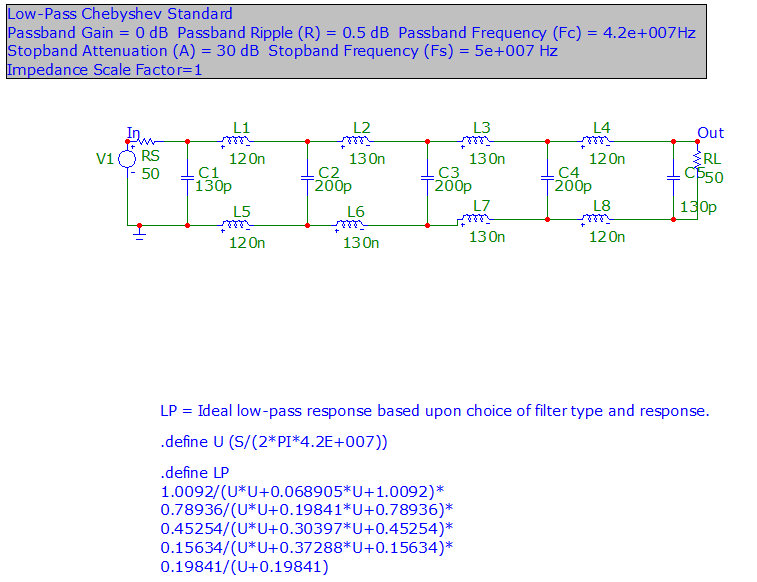
\includegraphics[width=0.8\linewidth]{Фильтр}
			\caption{Балансный фильтр низких частот}
			\label{fig:Бфильтр}
		\end{figure}
		
			
		\subsection{Цепи питания}
			\subsubsection{Выбор стабилизатора напряжения}
			Для выбора стабилизаторов напряжения рассчитаем все мощности источников питания:
			\begin{enumerate}
				\item АЦП --- напряжение питания составляет 3.3~В. при максимальном токе 70~мА., что даёт максимальную потребляемую мощность 231~мВт;
				\item Понижающий смеситель --- напряжение питания составляет 5~В. при максимальном токе 250~мА., что даёт максимальную потребляемую мощность 1250~мВт;
				\item МШУ --- напряжение питания составляет 2.5~В. при максимальном токе 25~мА., что даёт максимальную потребляемую мощность 62.5~мВт. на одно устройство. Общая потребляемая мощность всего тракта МШУ равна 187.5~мВт;
				\item УПЧ --- напряжение питания составляет 2.5~В. при максимальном токе 55~мА., что даёт максимальную потребляемую мощность 137.5~мВт. на одно устройство. Общая потребляемая мощность всего тракта УПЧ равна 275~мВт;
				\item ЦАП --- напряжение питания составляет 3.3~В. при максимальном токе 80~мА., что даёт максимальную потребляемую мощность 264~мВт;
				\item Повышающий смеситель --- напряжение питания составляет 5~В. при максимальном токе 205~мА., что даёт максимальную потребляемую мощность 1025~мВт;
				\item Оконечный смеситель --- напряжение питания составляет 5~В. при максимальном токе 90~мА., что даёт максимальную потребляемую мощность 450~мВт. на одно устройство. Общая потребляемая мощность всего тракта усилителя передатчика равна 900~мВт;
				\item Гетеродин --- напряжения питания составляют 5~В. при максимальном токе 65~мА. и 3.3~В. при максимальном токе 140~мА, что даёт максимальную потребляемую мощность 787~мВт:
			\end{enumerate}
		
			Далее рассчитаем мощность на каждом из питающий напряжений:
			
			\begin{itemize}
				\item 5~В: $ 1250 + 1025 + 900 + 325 = 3500 $~мВт;
				\item 3.3~В: $231 + 264 + 462 = 957 $~мВт;
				\item 2.5~В: $ 187.5 + 275 =  462.5 $~мВт.
			\end{itemize}
			
			Питание к ПП будет подводится 5~В лабораторным блоком питания с низким уровнем шумов и далее понижаться до 3.3~В и 2.5~В. 
			
			Понижение будет осуществляться линейными стабилизаторами LD1117~\cite{bib:Стабилизатор} c номинальным током 0.8~А, что полностью удовлетворяет требованиям по питанию 
			
			\subsubsection{Стандартная обвязка}
				Стандартная обвязка выбранного нами стабилизатора напряжения серии LD1117 представлена на рисунке~\ref{fig:обвязка:Стабилизатор}, полученном из документации~\cite{bib:Стабилизатор}. Данная схема включает в себя следующие компоненты:
				\begin{itemize}
					\item блокировочный конденсатор номиналом 0.1~мкФ.;
					\item сглаживающий конденсатор номиналом 10~мкФ.
				\end{itemize}
			
				Принципиальная схема полученного узла приведена в приложении~\ref{app:SCH} на листе 9.
				\begin{figure}[h!]
					\centering
					\includegraphics[width=0.7\linewidth]{"Обвязка стабилизатора"}
					\caption{Стандартная обвязка стабилизатора}
					\label{fig:обвязка:Стабилизатор}
				\end{figure}
			
	\pagebreak
	
	\section{Выбор конструктивных решений ПП}
	
		\subsection{Аналоговый тракт}
			Для правильного согласования и отсутствия отражений выберем полосковый волновод на частотах 4,9-5~Ггц. Для расчета будем использовать систему расчету встроенную в KiKad. Она работает по формулам представленным в литературе \cite{bib:СВЧ}. Как видно на рисунке~\ref{fig:волновод5} получившиеся параметры для платы на FR4 составляют:
			\begin{itemize}
				\item ширина дорожки $W~=~0,822291~mm $;
				\item расстояние до внешнего полигона $ S~=~2~mm $;
				\item толщина печатной платы $ H~=~0,8~mm$.
			\end{itemize} 
		 
			\begin{figure}[h!]
				\centering
				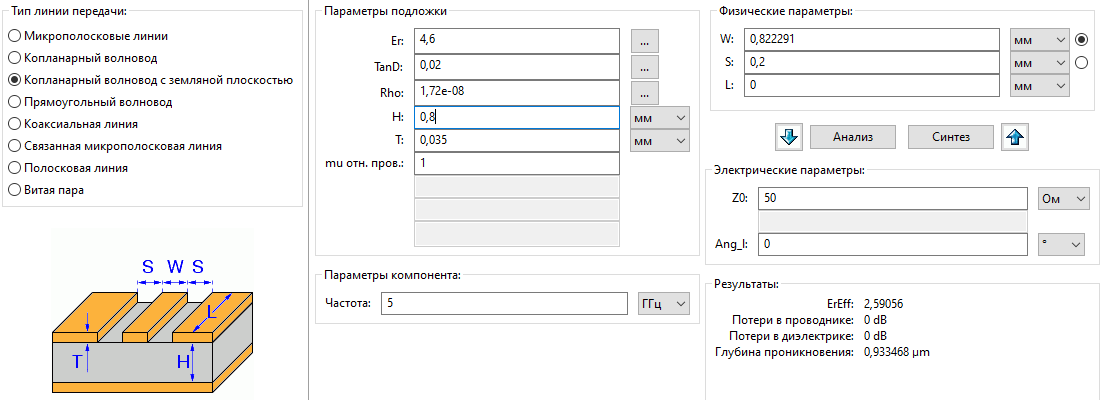
\includegraphics[width=0.9\linewidth]{Волновод}
				\caption{Параметры компланарного волновода с земляной плоскостью}
				\label{fig:волновод5}
			\end{figure}
			Для балансной линии на 5~Ггц обеспечим минимальное различие длин дрожек рисунок \ref{fig:Длинна}.
			\begin{figure}[h!]
				\centering
				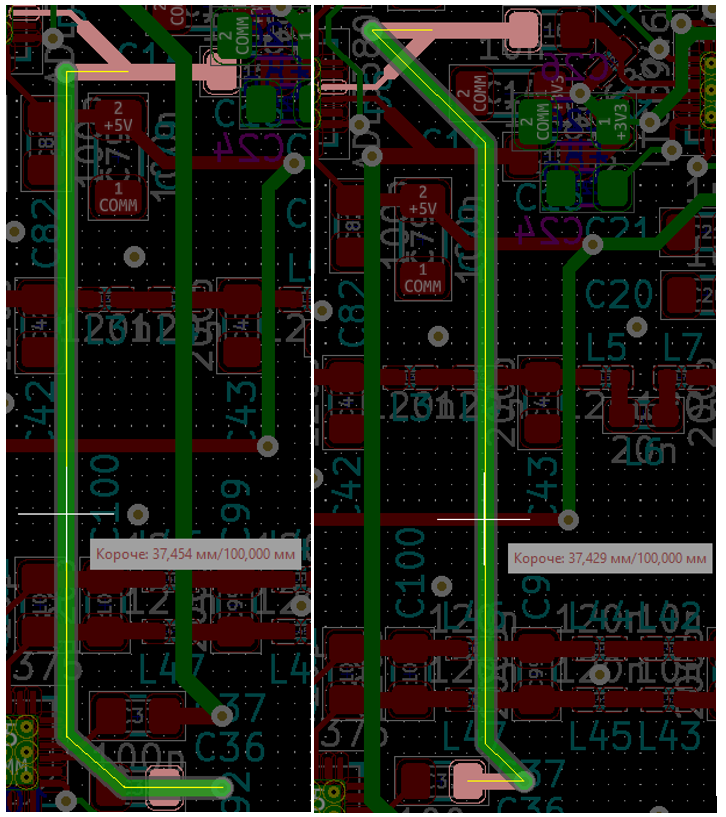
\includegraphics[width=0.7\linewidth]{Длинна}
				\caption{Размер балансной линии, идущей от генератора к повышающему смесителю}
				\label{fig:Длинна}
			\end{figure}
			
		\subsection{Цифровой интерфейс}
		Рассчитаем разность длин дорожек для цифрового сигнала 100~МГц итоговые данные представлены на рисунке~\ref{fig:Волновод100} . Так как у нас цифровой сигнал поиступает с параллельного выхода АЦП то его не правильное детектирование будет производится при сдвиге фаз между битами в 90 градусов. Следовательно критическая разность длинн составляет $466~mm$, дорожки попадают в заданный интервал (рисунок~\ref{fig:цифра}).
		
	
		
		\begin{figure}[h!]
			\centering
			\includegraphics[width=0.9\linewidth]{"Волновод 100Мгц"}
			\caption{Результаты расчета для проводников 100МГц}
			\label{fig:Волновод100}
		\end{figure}
	
		\begin{figure}[h!]
			\centering
			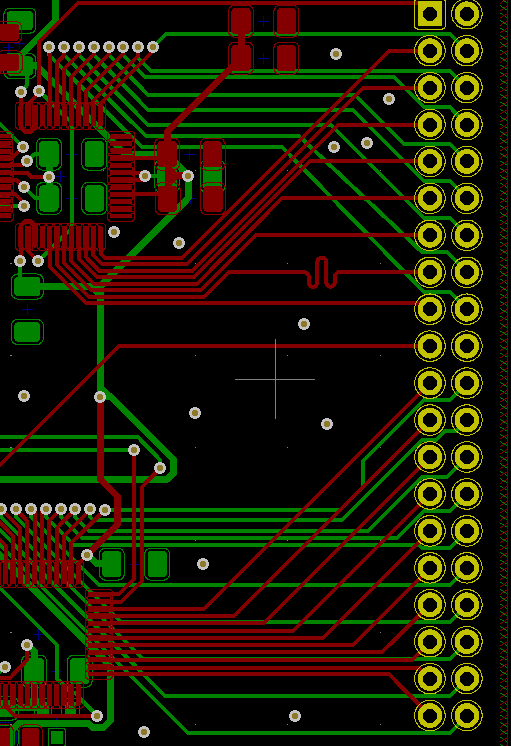
\includegraphics[width=0.5\linewidth]{Цифвх-вых}
			\caption{Выход и вход АЦП и ЦАП}
			\label{fig:цифра}
		\end{figure}
			
			Для считывания и передачи данных использован коннектор с шагом пина $2,54~mm$. Данное решение обусловлено использованием в качестве отладочной платы "QMTECH Cyclone IV Starter Kit" показанной на рисунке~\ref{fig:ПЛИС}.
		\begin{figure}[h!]
			\centering
			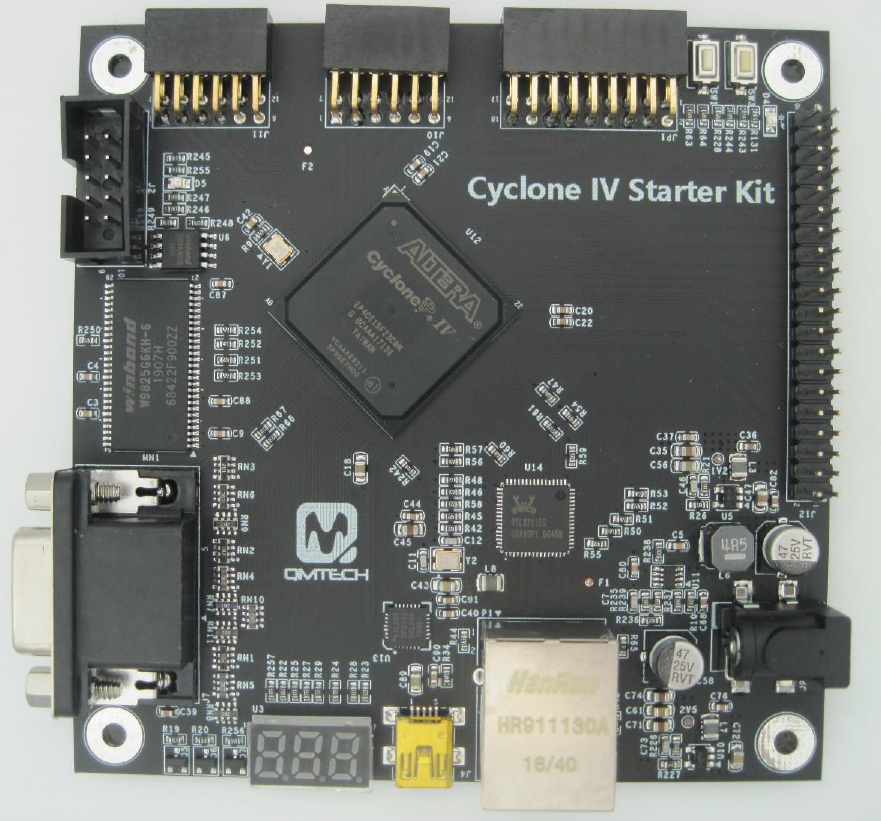
\includegraphics[width=0.5\linewidth]{ПЛИС}
			\caption{Отладочная плата QMTECH Cyclone IV Starter Kit}
			\label{fig:ПЛИС}
		\end{figure}
		\subsection{Цепи питания}
		Выберем толщину цепи питания исходя из теоретической мощности равной 5~Вт, а значит ток равен 1~А при питающем напряжении 5~В. Воспользуемся встроенным калькулятором в KiKad рисунок~\ref{fig:Дорожка}. Выбираем толщину дорожки с запасом. Итого толщина питания выбрана $0.5~mm $.На рисунке~\ref{fig:Питание} приведен вид цепей питания на плате.
		\begin{figure}[h!]
			\centering
			\includegraphics[width=0.9\linewidth]{"Расчет минимальной толщины дорожки"}
			\caption{Рассчет минимальной толщины дорожки}
			\label{fig:Дорожка}
		\end{figure}
		 \begin{figure}[h!]
		 	\centering
		 	\includegraphics[width=0.3\linewidth]{"Система питания"}
		 	\caption{Размещение цепи питания на печатной плате}
		 	\label{fig:Питание}
		 \end{figure}
		 
		\subsection{Определение класса ПП}
		Для определения класса печатной платы рассмотрим классы цепей, использованных в данной ПП, которые показаны на рисунке~\ref{fig:классы цепей}.
		\begin{figure}[h!]
			\centering
			\includegraphics[width=0.7\linewidth]{"Класс цепей"}
			\caption{Все классы цепей использованных в разводке печатных плат}
			\label{fig:классы цепей}
		\end{figure}
	
		Из таблицы классов выберем класс печатной платы. По характеристикам плата относится к 5 классу.
		
		\begin{figure}[h!]
			\centering
			\includegraphics[width=0.7\linewidth]{"Класс печатных плат"}
			\caption{Класс печатной платы}
			\label{fig:Класс}
		\end{figure}
		
		Так же приведем модели полученной ПП на рисунках~\ref{fig:sdrb}~и~\ref{fig:sdrt}. Полная КД на ПП приведена в приложении~\ref{app:PCB}.
		\begin{figure}[h!]
			\centering
			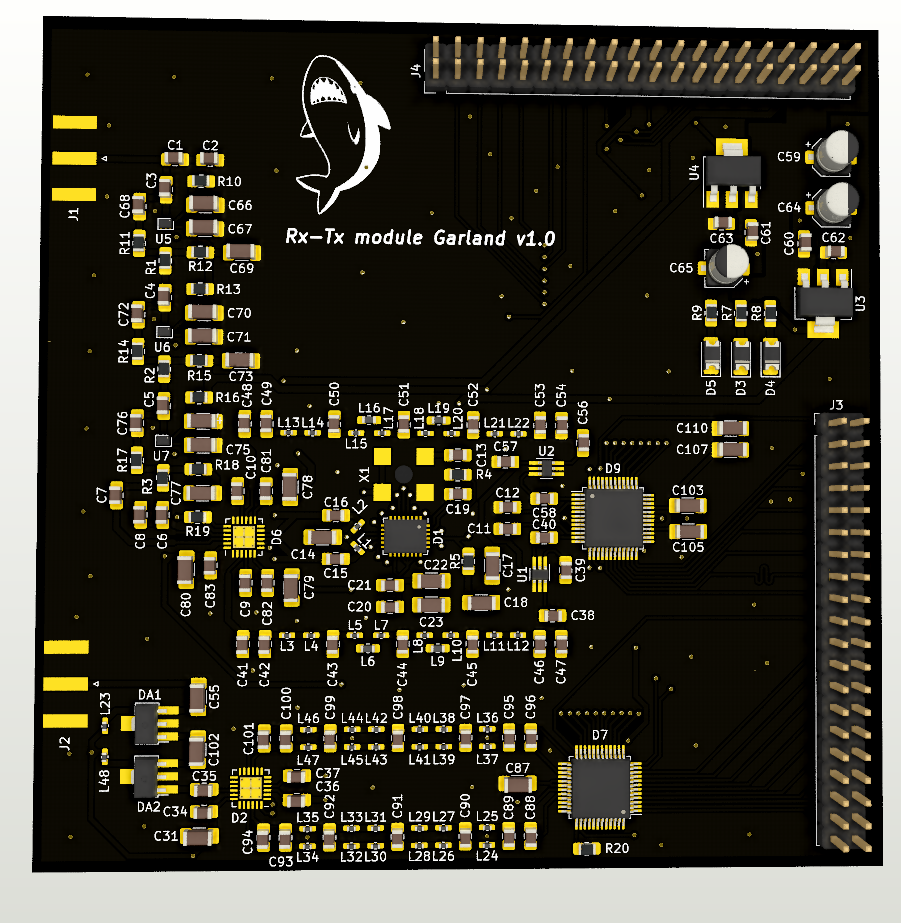
\includegraphics[width=0.6\linewidth]{SDRтоп}
			\caption{Верхний слой ПП}
			\label{fig:sdrt}
		\end{figure}
		\begin{figure}[h!]
			\centering
			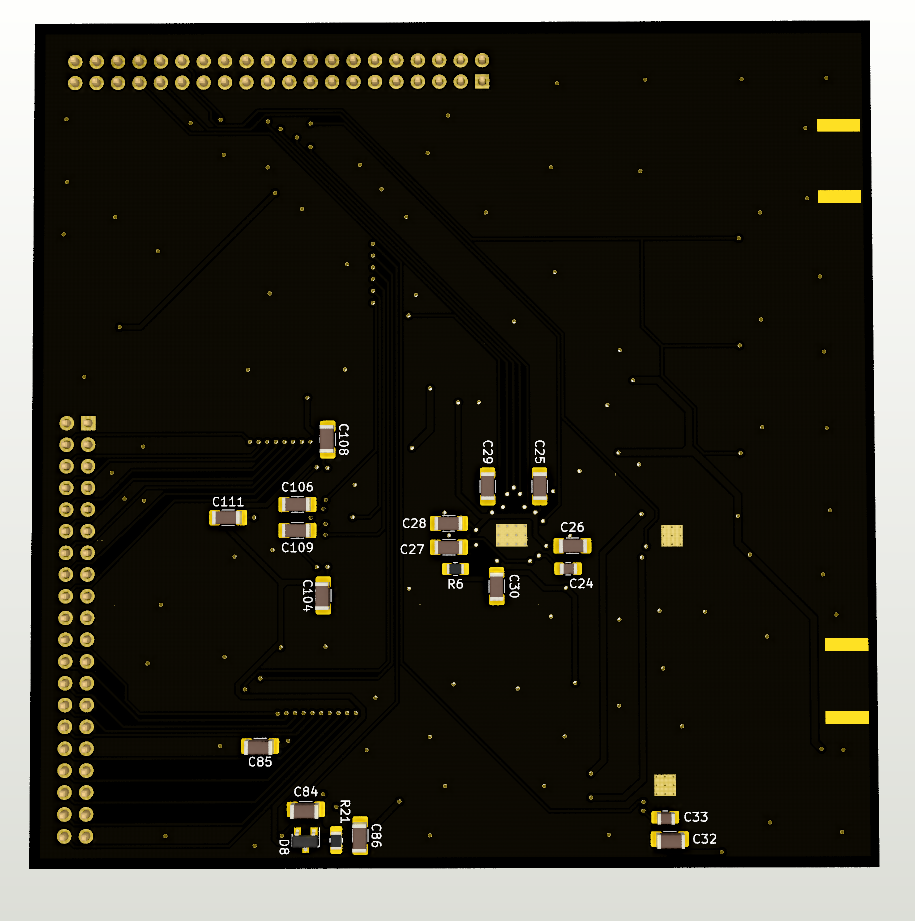
\includegraphics[width=0.6\linewidth]{SDRбот}
			\caption{Нижний слой ПП}
			\label{fig:sdrb}
		\end{figure}
		
		
		
		
	\pagebreak 
	
	\quad
	
	\newpage 
	\section*{ЗАКЛЮЧЕНИЕ}
	\addcontentsline{toc}{section}{ЗАКЛЮЧЕНИЕ}
	
	Целью данной работы была реализация приемо-передающей ячейки для построения на ее основе более сложную систему - приемо-передающий модуль в приложении~\ref{app:Структурная схема модуля}. График дальнейших работ приведен на рисунке Преимуществами данной ячейки являются низкая стоимость и рабочая полоса. Это позволит провести первичные эксперименты и определить конструктивные и иные недочеты в данном прототипе. По результатам испытаний будут внесены правки в данную РПЗ. В качестве приемной и передающей антенны будет использована патч антенна реализованная в качестве курсовой работы <<Проектирование и моделирование
	сверхширокополосной печатной антенной решетки>> выполненной студентом Потаповым Дмитрием Александровичем. 
	
	\begin{figure}[h!]
		\centering
		\includegraphics[width=0.7\linewidth]{"План работ"}
		\caption{План работ включает в себя реализацию модуля в качестве курсовой "Проектировани радиоэлектронного устройства",а так же реализацию всего комплекса в качестве выпускной квалификационной работы}
		\label{fig:План работ}
	\end{figure}
	
	\pagebreak
	

	
	
	\begin{thebibliography}{3}
	\addcontentsline{toc}{section}{СПИСОК ИСПОЛЬЗОВАННЫХ ИСТОЧНИКОВ}
		\bibitem{bib:АЦП}
		https://www.analog.com/media/en/technical-documentation/data-sheets/AD9288.pdf Дата~обращения:~22.12.2020
		\bibitem{bib:ПонижающийСмеситель}
		https://www.analog.com/media/en/technical-documentation/data-sheets/ADL5380.pdf Дата~обращения:~22.12.2020
		\bibitem{bib:МШУ}
		https://www.nxp.com/docs/en/data-sheet/BGU7003W.pdf Дата~обращения:~22.12.2020
		\bibitem{bib:УПЧ}
		https://www.nxp.com/docs/en/data-sheet/BGA2874.pdf Дата~обращения:~22.12.2020
		\bibitem{bib:ЦАП}
		https://www.analog.com/media/en/technical-documentation/data-sheets/ADV7123.pdf Дата обращения: 22.12.2020
		\bibitem{bib:ПовышающийСмеситель}
		https://www.analog.com/media/en/technical-documentation/data-sheets/ADL5375.pdf Дата обращения: 22.12.2020
		\bibitem{bib:ОконечныйУсилитель}
		https://cdn1.components.ru/174/210174.pdf Дата~обращения:~22.12.2020
		\bibitem{bib:Стабилизатор}
		http://www.st.com/st-web-ui/static/active/en/resource/technical/document/ datasheet/CD00000544.pdf Дата~обращения:~22.12.2020
		\bibitem{bib:Генератор}
		https://www.analog.com/media/en/technical-documentation/data-sheets/6946fb.pdf Дата~обращения:~22.12.2020
		\bibitem{bib:СВЧ}
		http://venec.ulstu.ru/lib/2002/1/SVCH.pdf Дата~обращения:~22.12.2020

	\end{thebibliography}
	
	\pagebreak
	
	\appendix
	\titleformat{\section}[display]
	{\normalfont\Large\bfseries}
	{\centering Приложение\ \thesection\\(справочное)}
	{0pt}{\Large\centering}
	\renewcommand{\thesection}{\Asbuk{section}}
	
	\section{Структурная схема РЧ модуля}\label{app:Структурная схема модуля}
	\pagebreak
	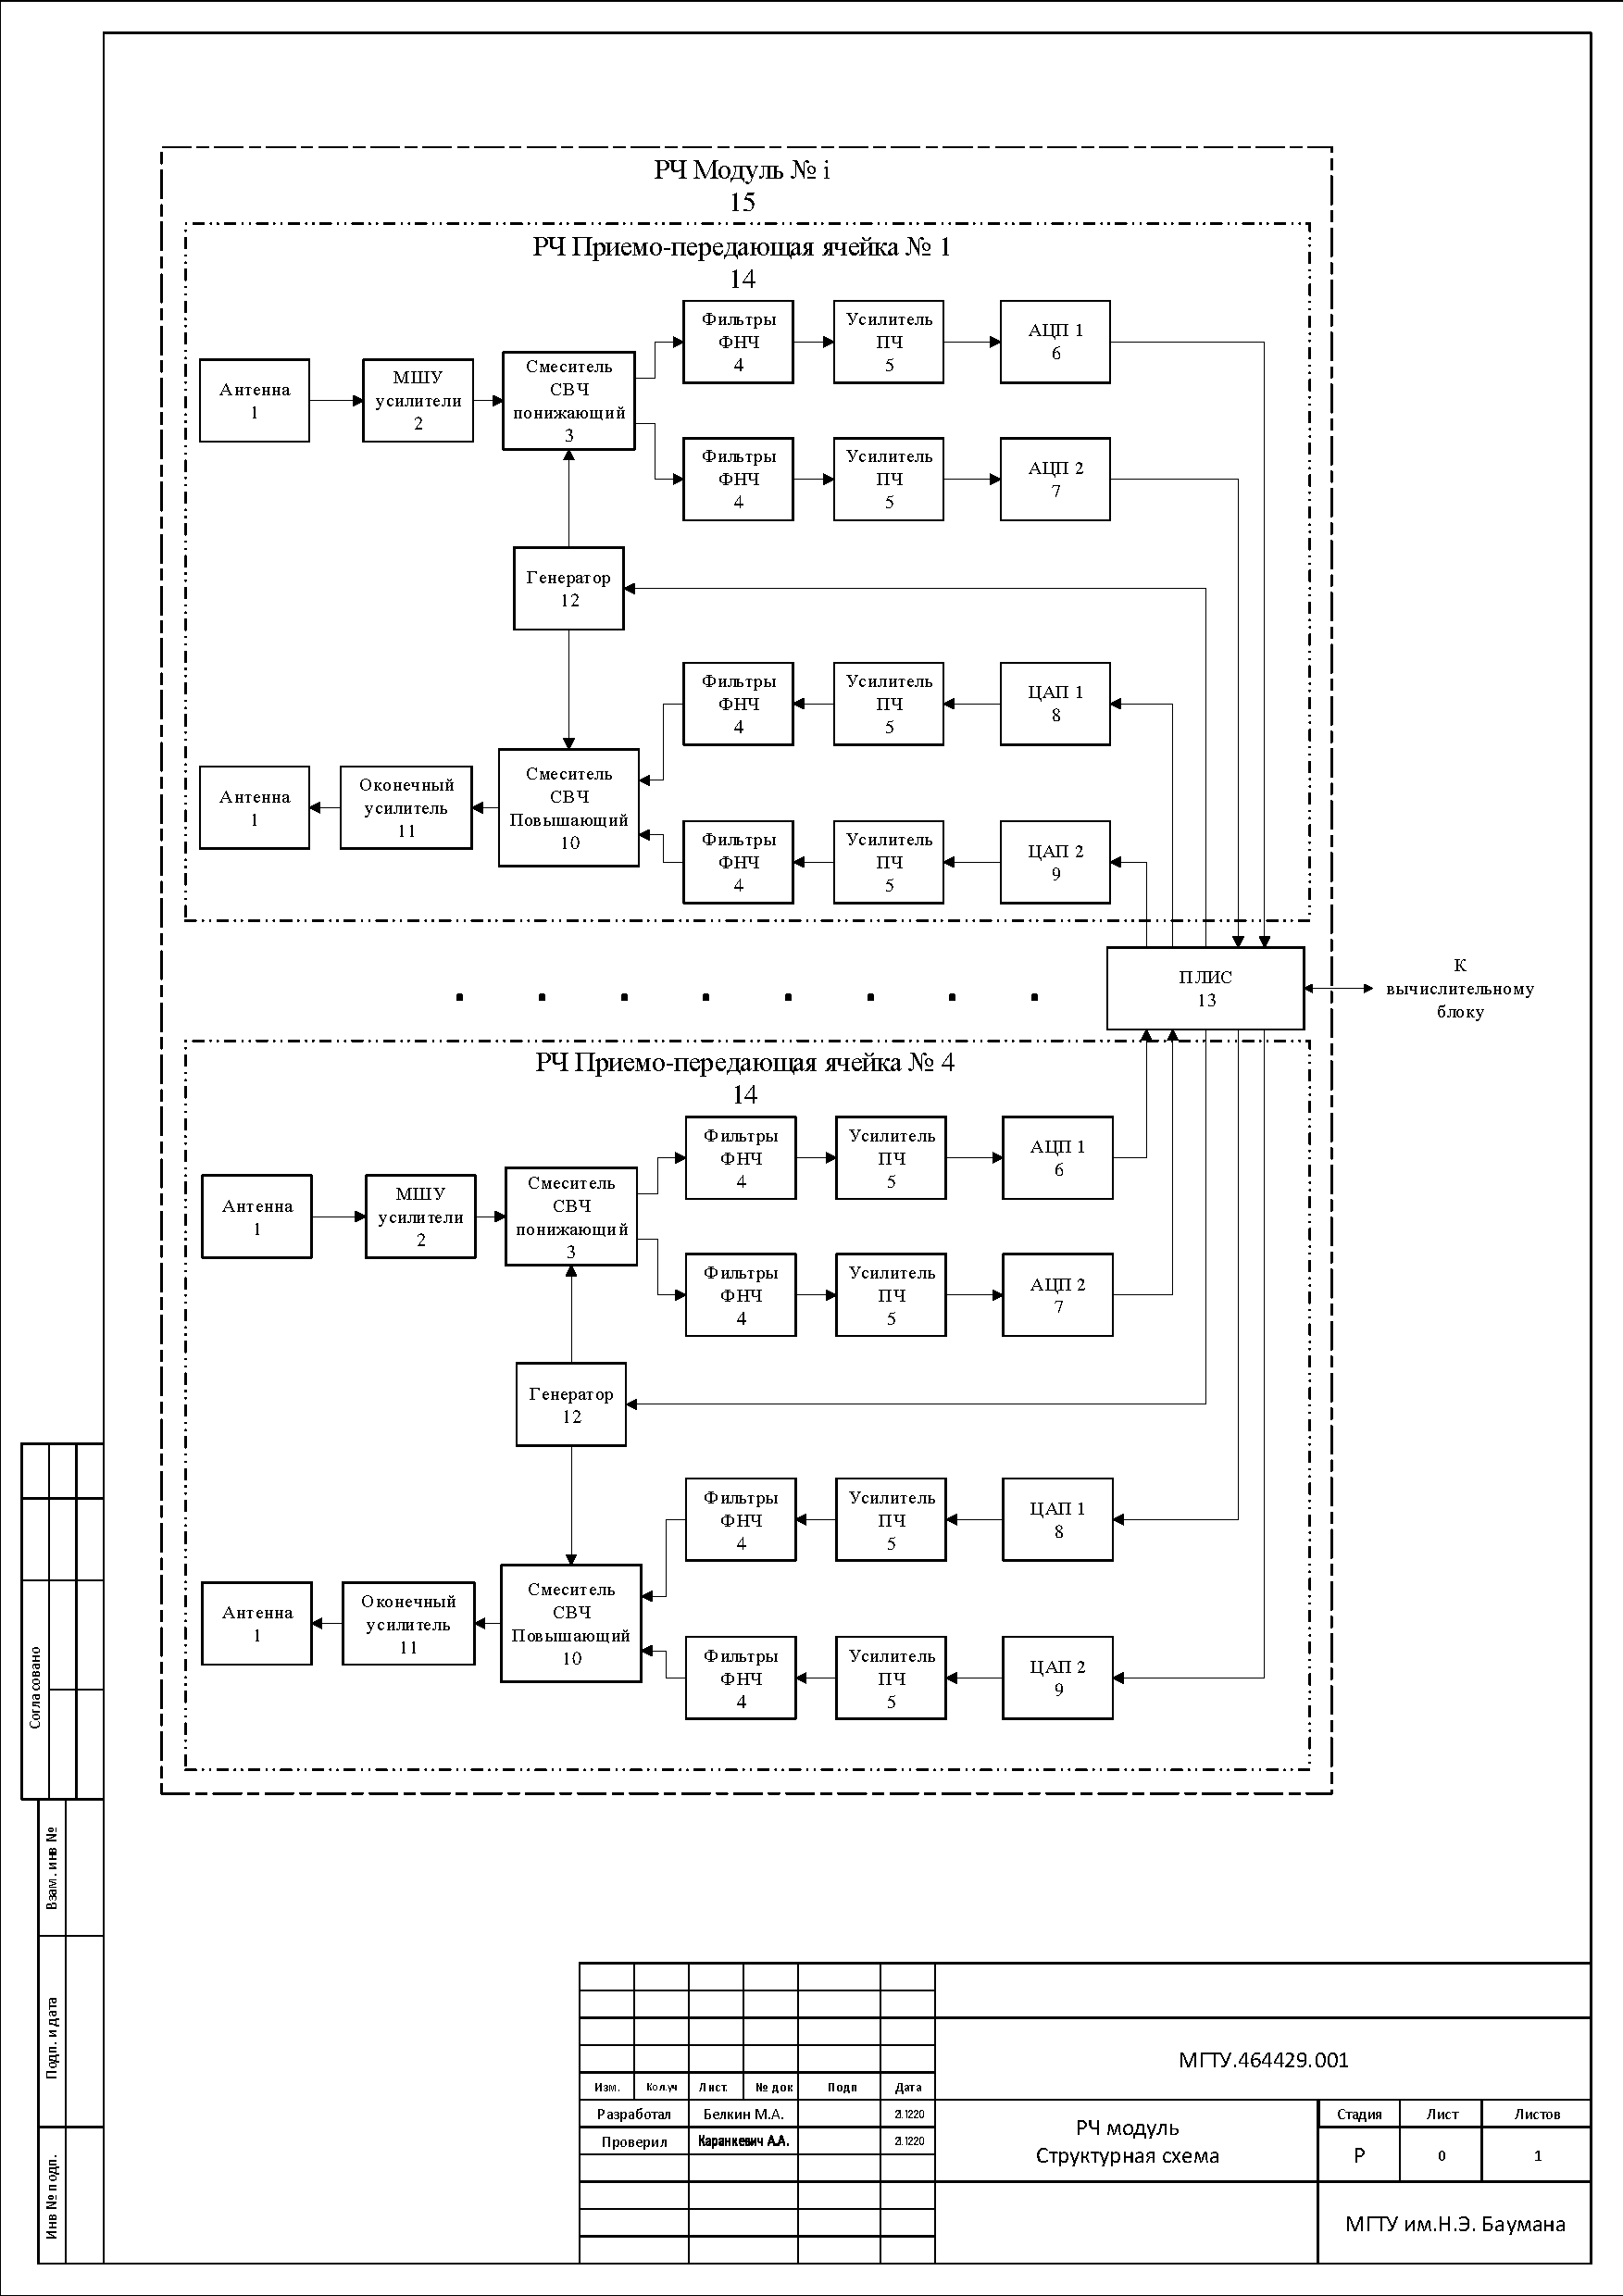
\includepdf[pages=-,fitpaper]{Структурная схема модуля.pdf}
	\pagebreak
	
	\section{Структурная схема ПЛИС}\label{app:Структурная схема ПЛИС}
	\pagebreak
	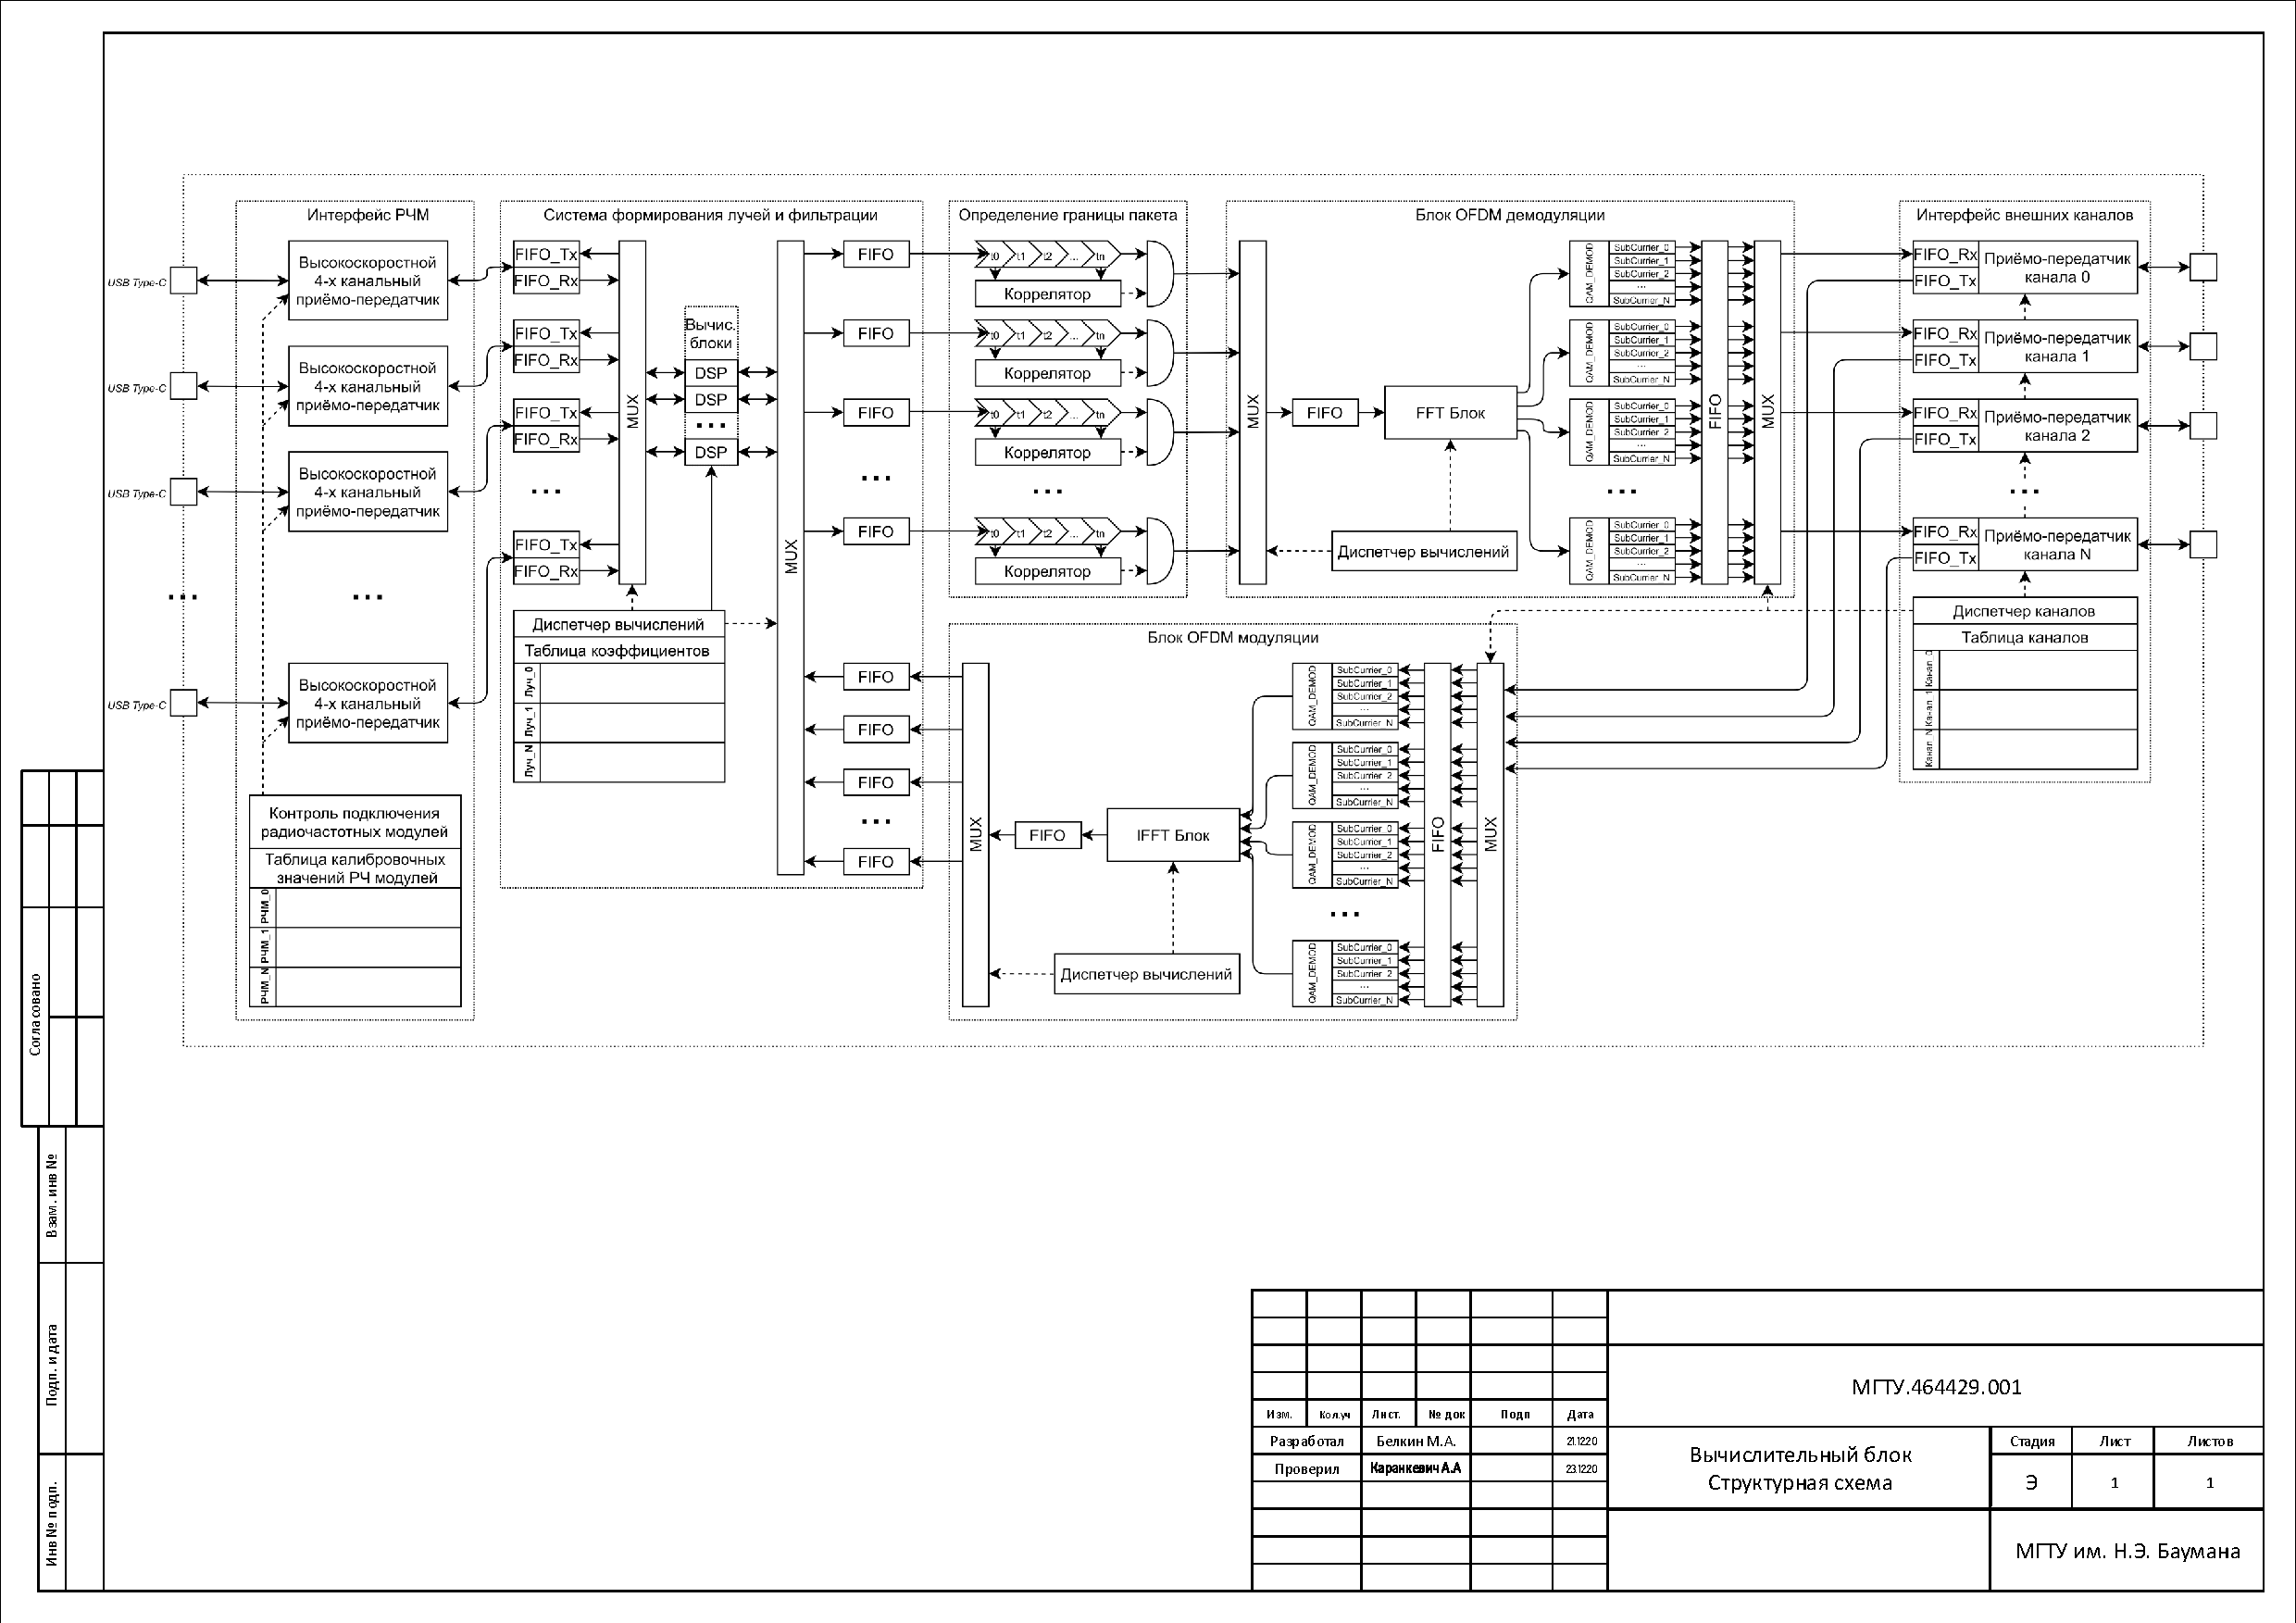
\includepdf[landscape=true,pages=-,fitpaper]{Структурная схема ПЛИС.pdf}
	\pagebreak
	
	\section{Принципиальная схема ППМ}\label{app:SCH}
	\pagebreak

	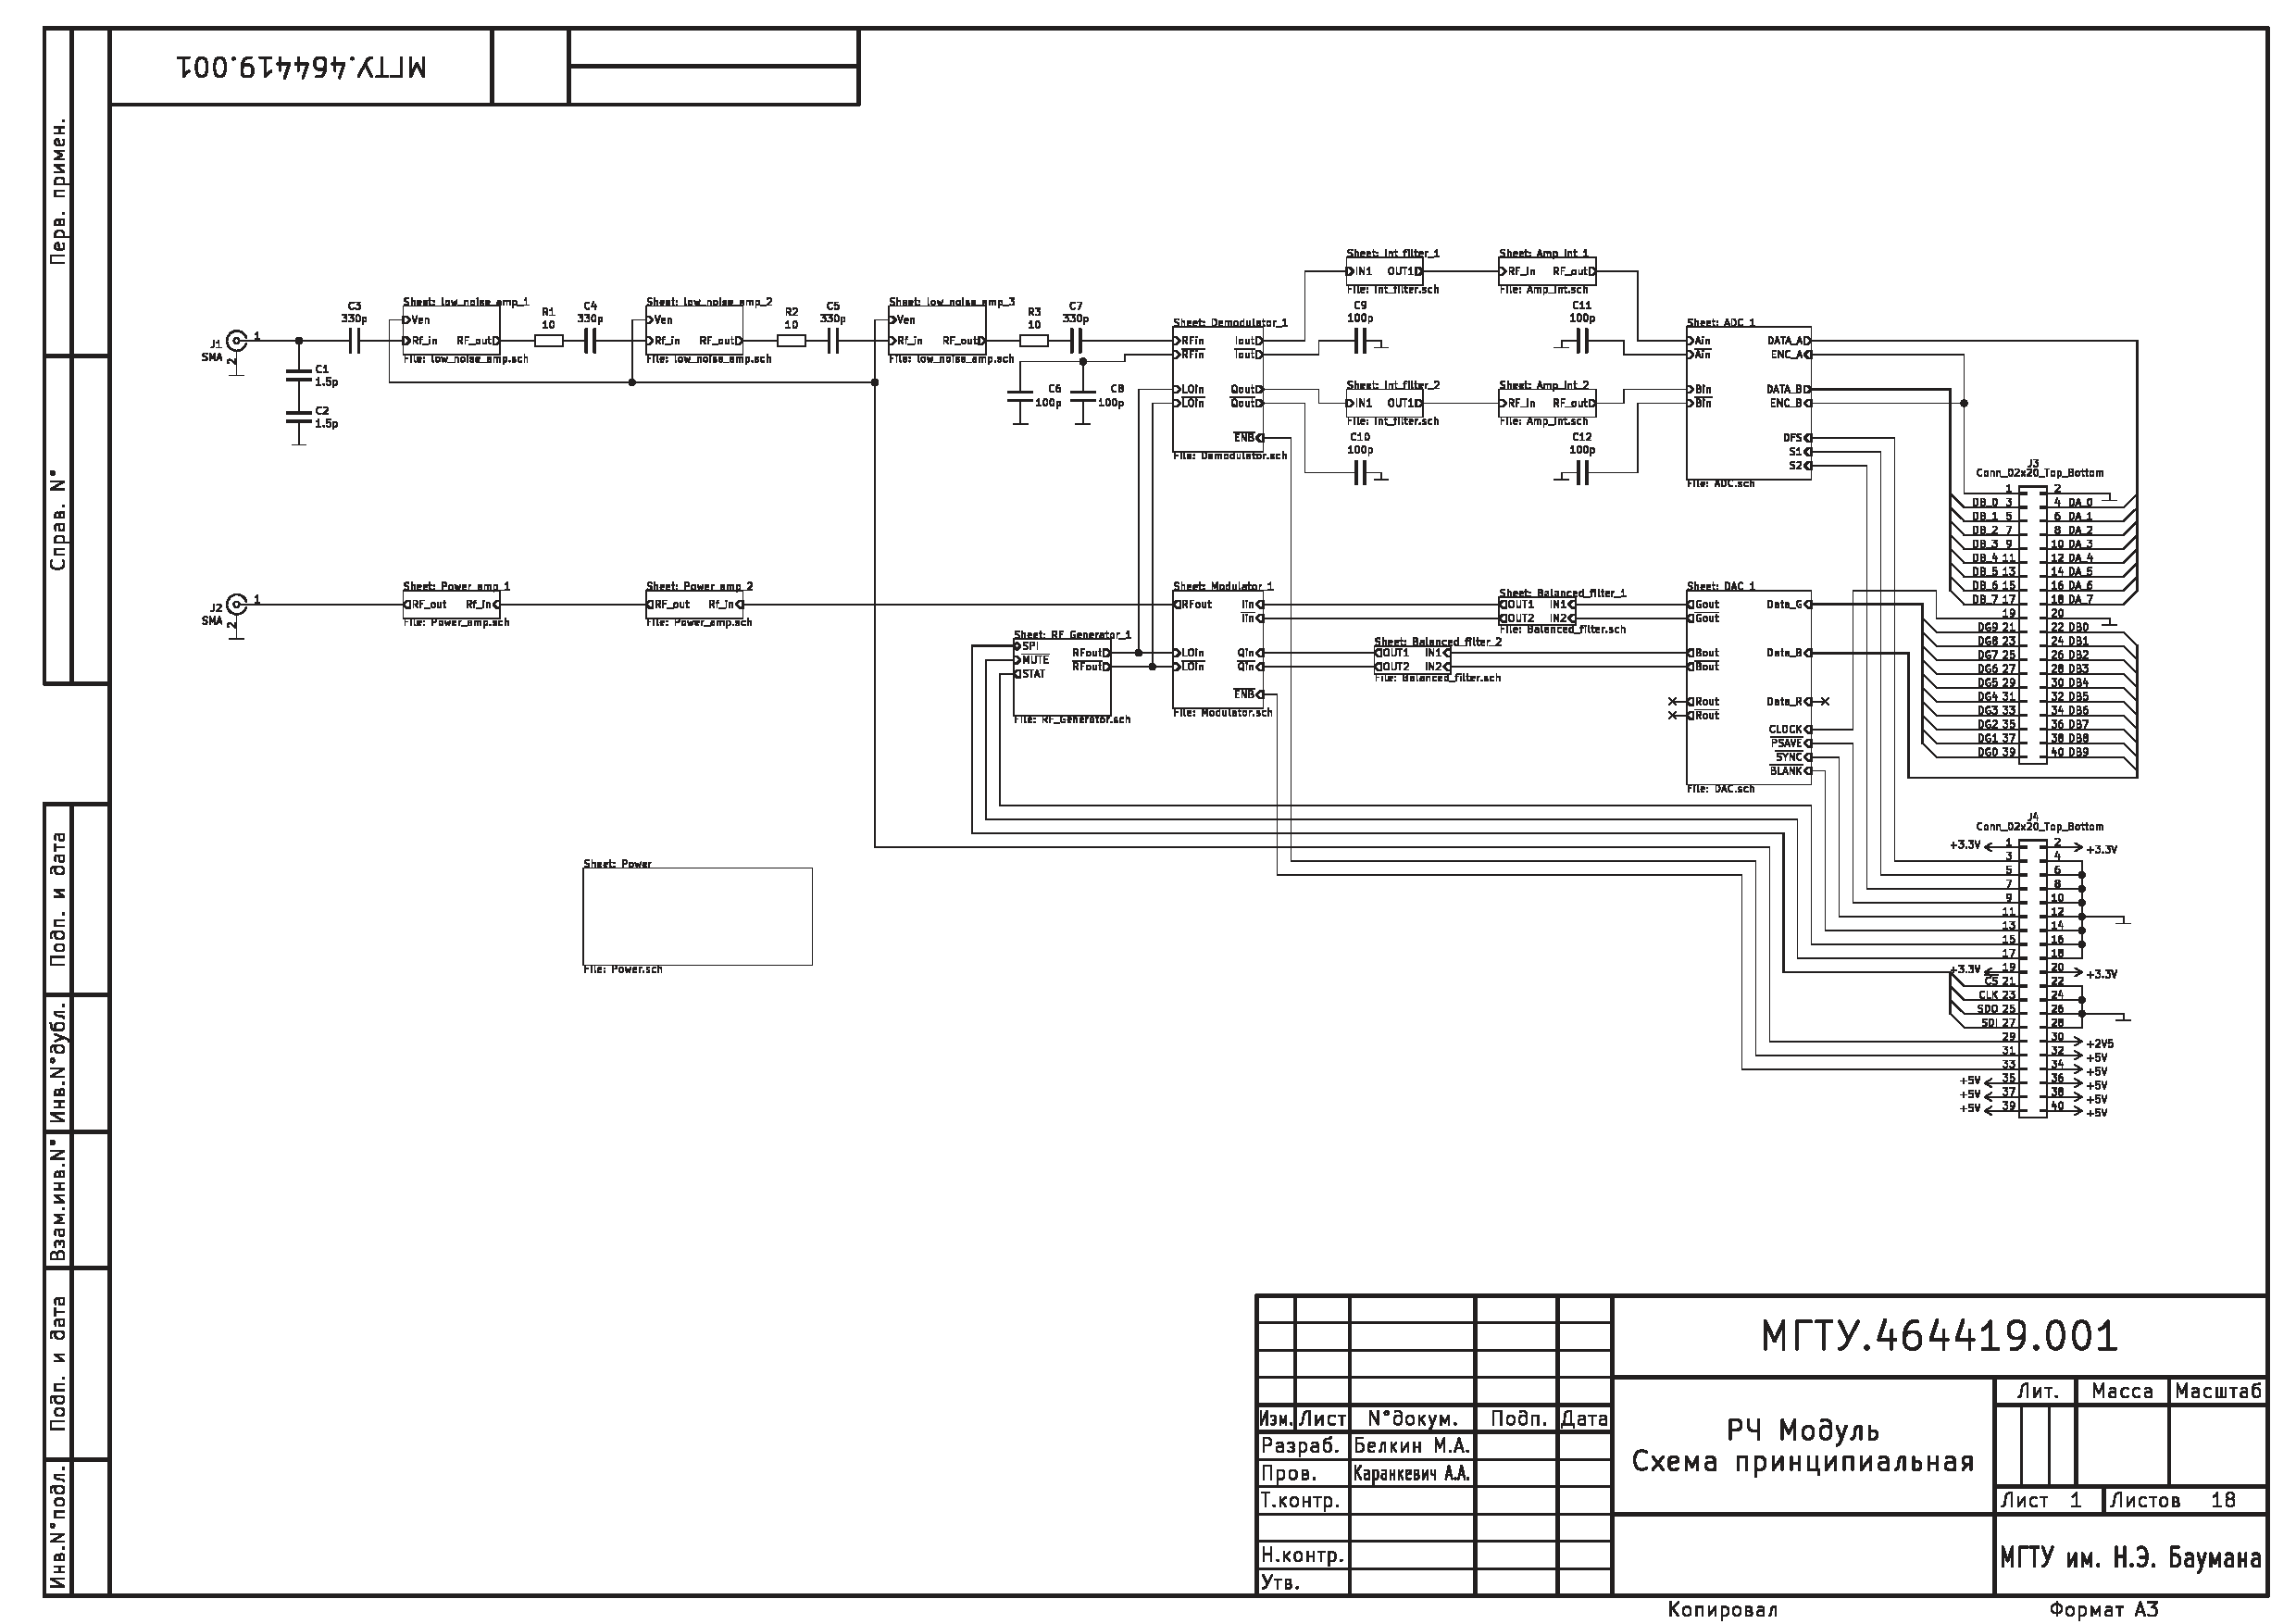
\includepdf[landscape=true,pages=-,fitpaper]{SDR-Sch-title.pdf}
	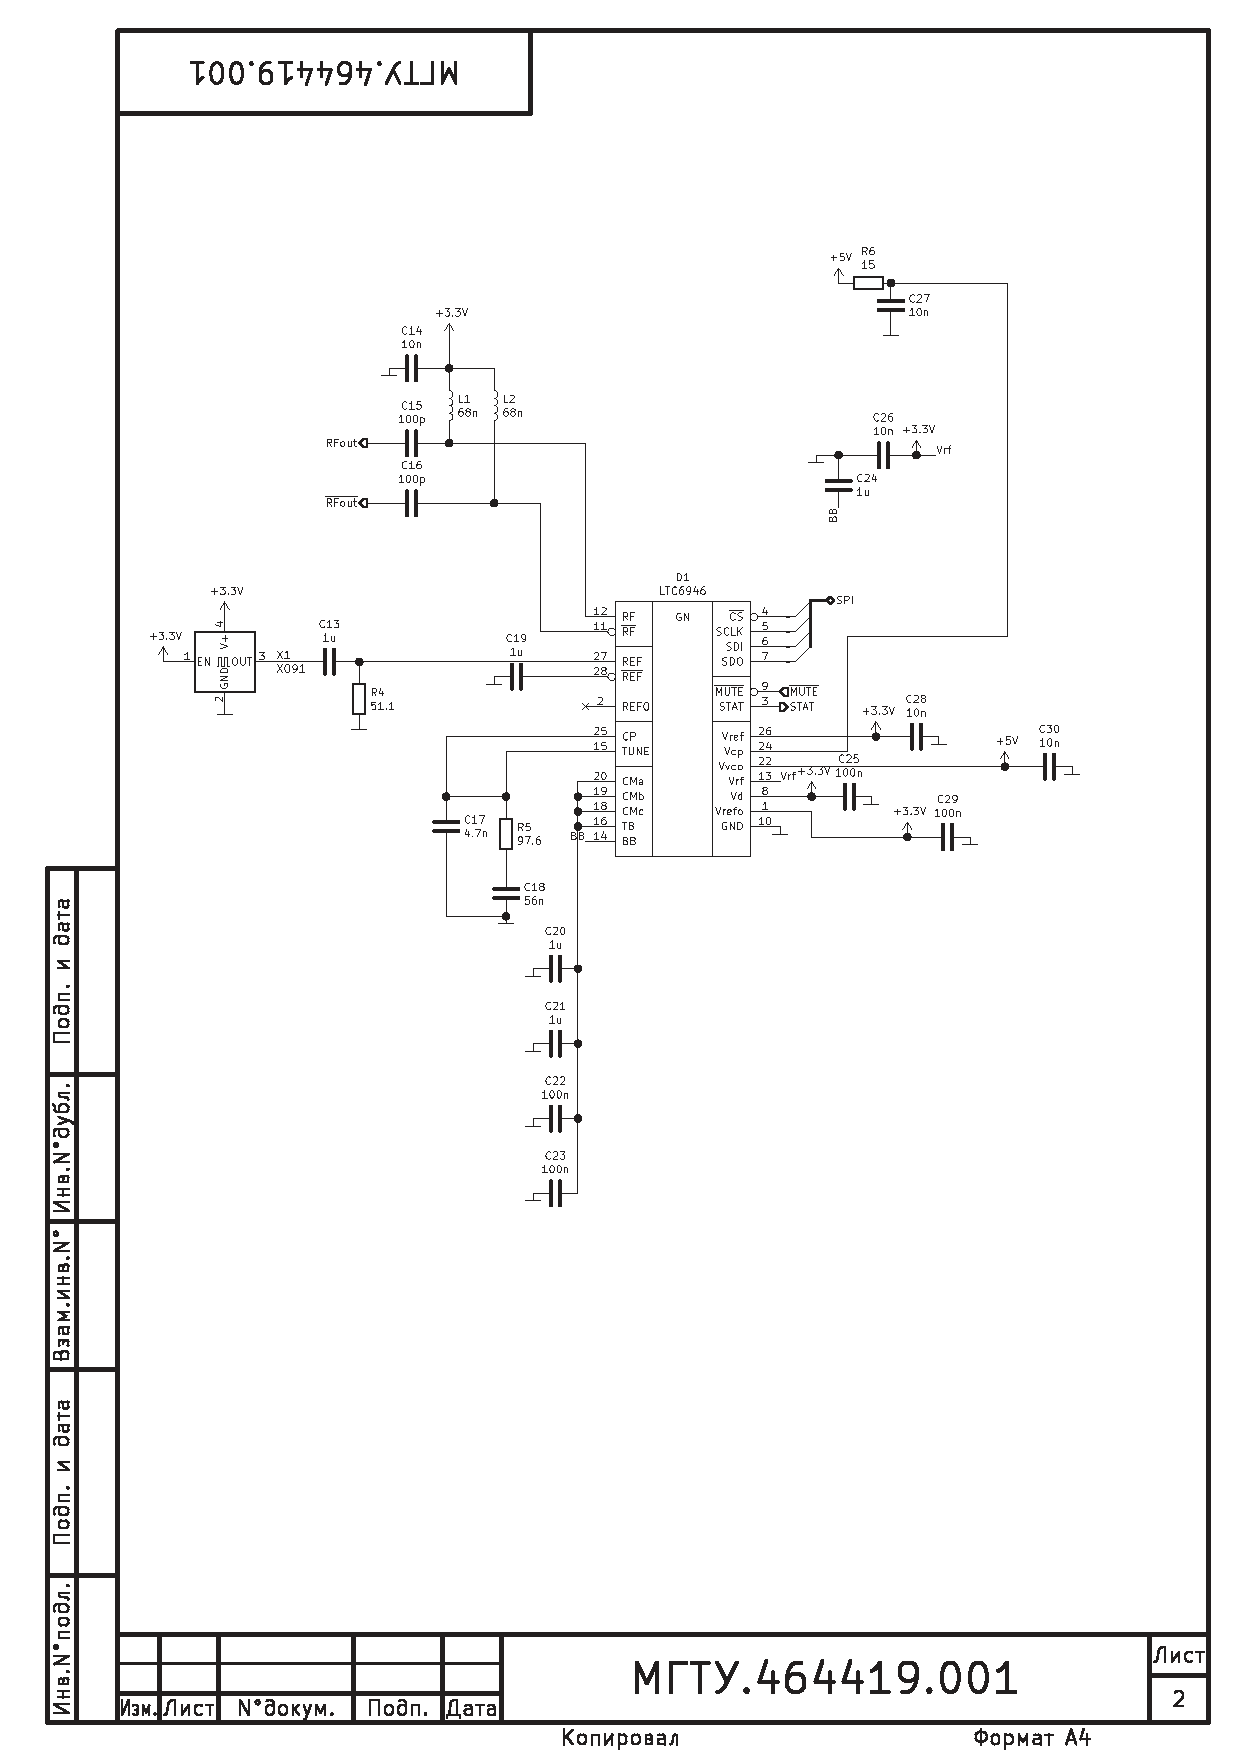
\includepdf[pages=-]{SDR-Sch.pdf}
	
	\pagebreak
	
	\section{PCB схема ППМ}\label{app:PCB}
	\pagebreak
	
	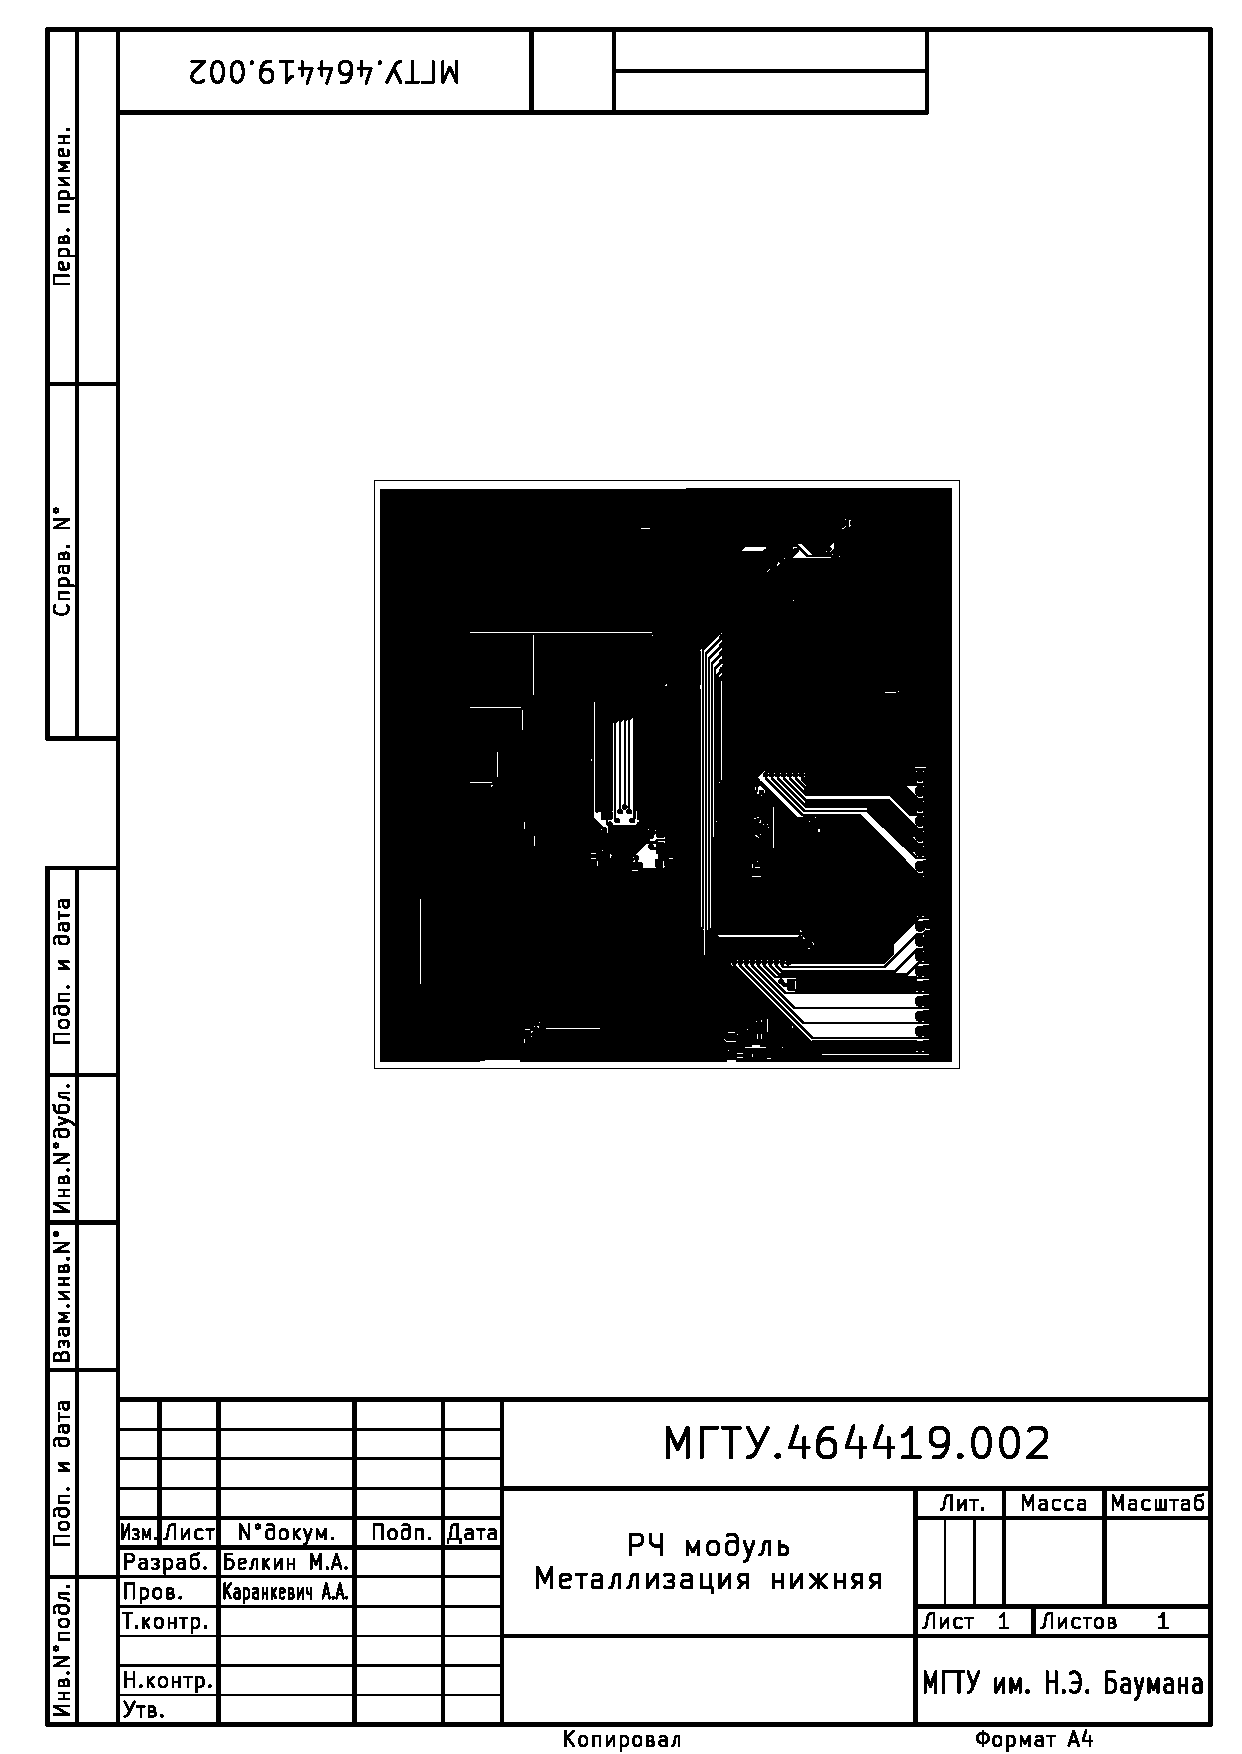
\includepdf[pages=-]{SDR-PCB.pdf}
	
	\pagebreak

\end{document}